\chapter{Designing the System}
	In the following chapter, the overall design of the system is discussed. First and foremost, the basic architecture is decided, based on the requirements described in section \ref{sec:requirements} on page \pageref{sec:requirements}. Then more detailed subjects are covered, such as how authentication will work, how the solution keeps the users' data safe, and generally how it will work under the hood - so to speak.

	\section{Architecture}
		\label{sec:arch}
		As per the requirements specified in section \ref{sec:requirements} on page \pageref{sec:requirements} the solution will have to be distributed. As such, there are two primary basic paradigms which can be used: Peer-to-Peer and Client-Server. In the following sections the pros and cons of the two will be discussed, and a conclusion of which is more beneficial for the project will be made.

		\begin{figure}[p]
			\centering
			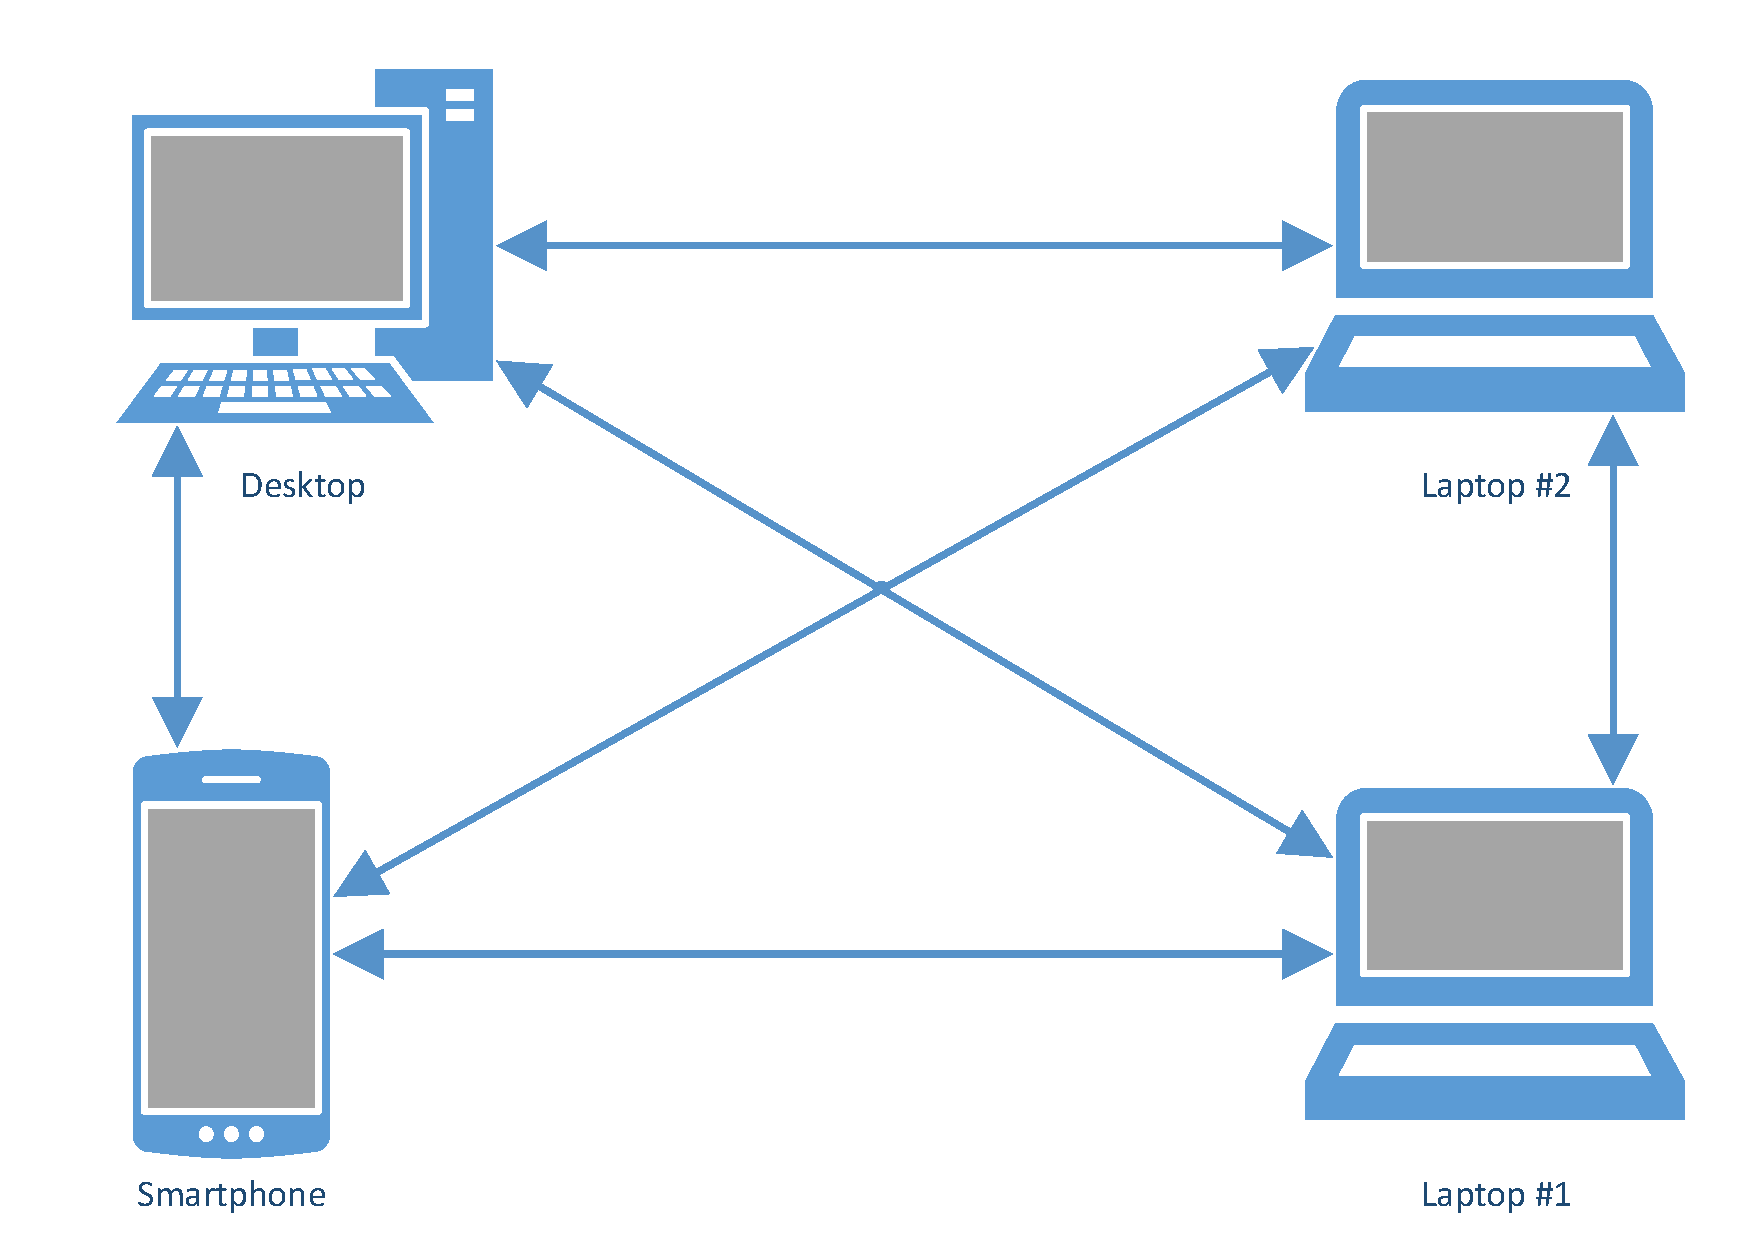
\includegraphics[width=0.8\textwidth]{figures/design/PeerToPeer.pdf}
			\caption{Peer-to-Peer structure visualised.}
			\label{fig:peertopeer}
		\end{figure}

		\begin{figure}[p]
			\centering
			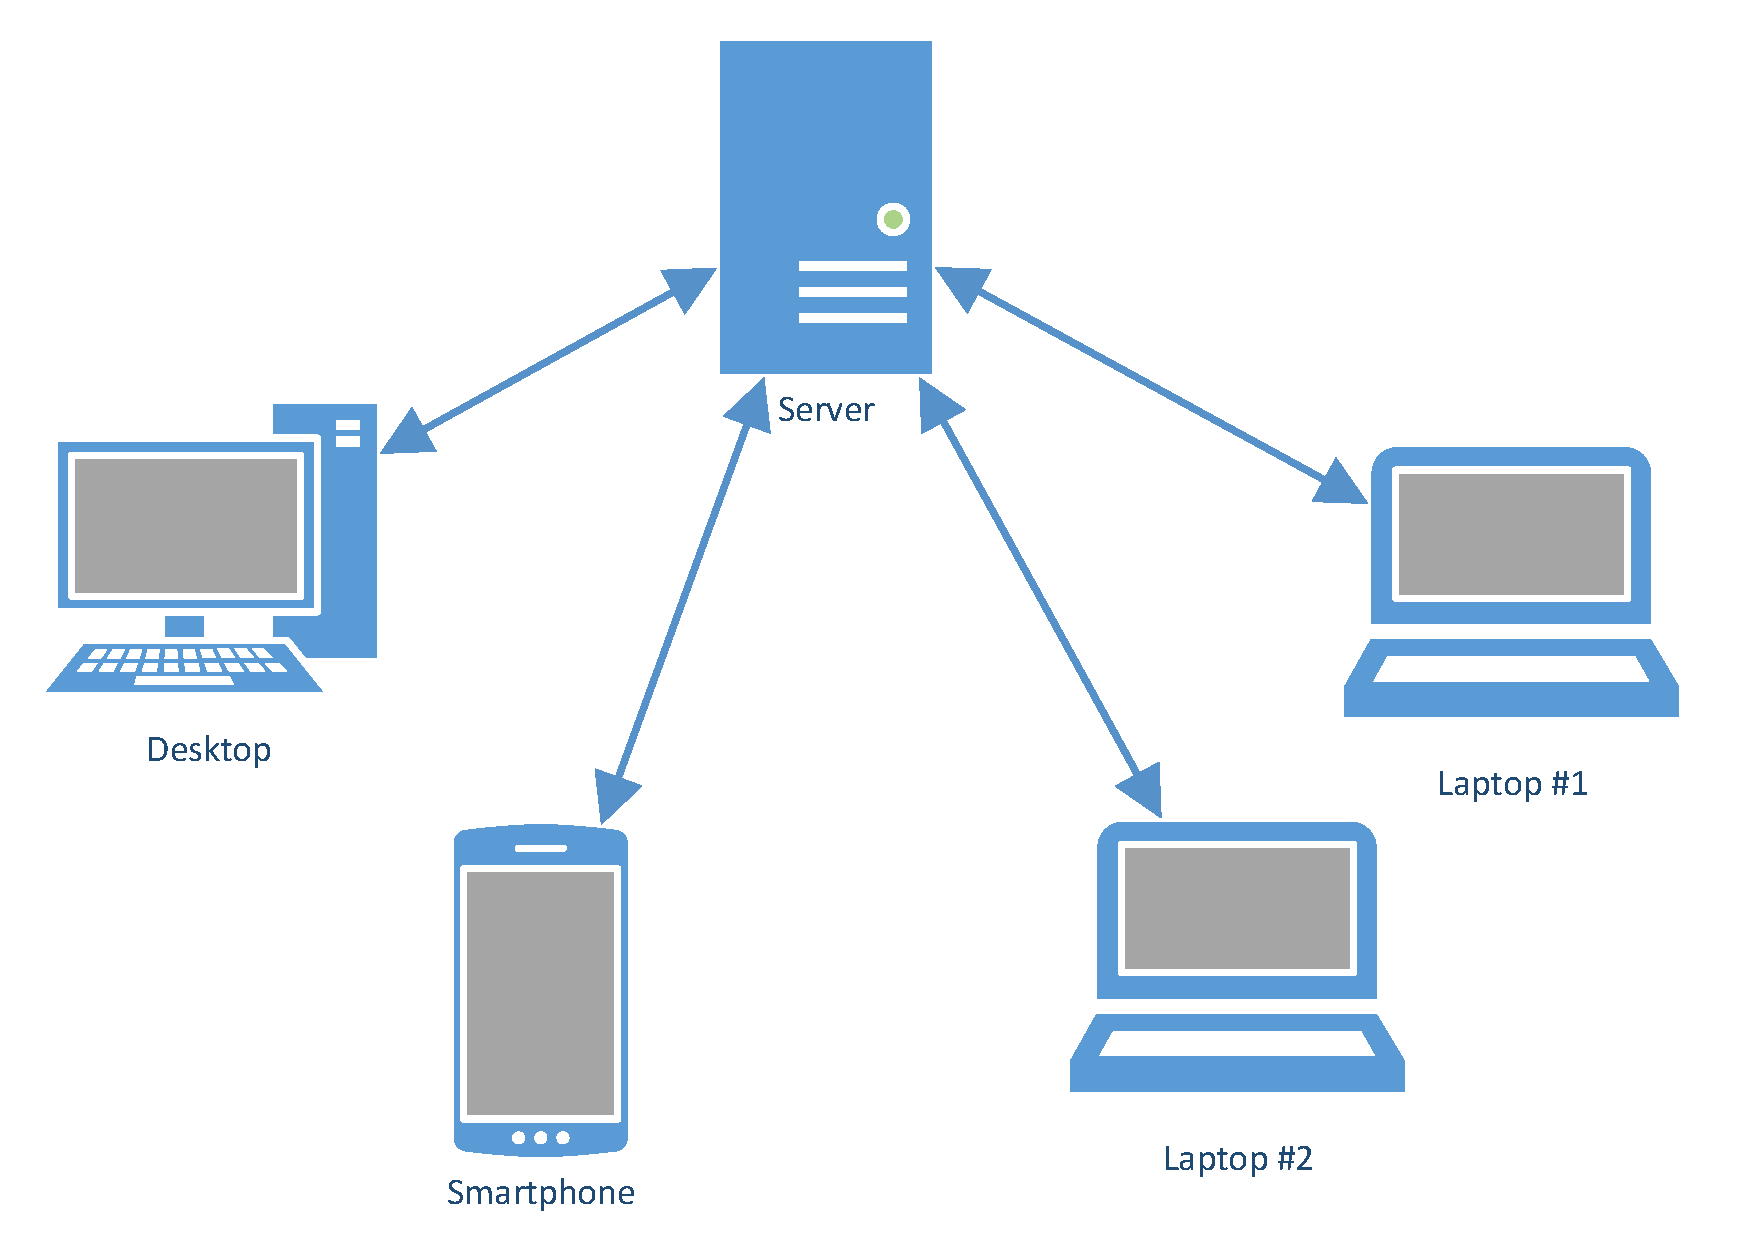
\includegraphics[width=0.8\textwidth]{figures/design/ClientServer.pdf}
			\caption{Client-Server structure visualised.}
			\label{fig:clientserver}
		\end{figure}


		\subsection{Peer-to-Peer}
			Over the past few years, peer-to-peer technology has become ever so more appealing to the masses. Applications such as BittorrentSync applies peer-to-peer technology in an effort to synchronise data between devices. Such an approach could easily be adapted to the problem at hand. A number of a user's devices are online, and synchronises a local password database file between themselves, as visualised on figure \ref{fig:peertopeer} on page \pageref{fig:peertopeer}. This file is then accessed through a native application, on the target device. 

			This approach \emph{definitely} has the lowest overhead of the two: After all it is only devices that needs to have access to the passwords, that need to be setup, maintained, and running for it to be used. However, it does have some drawbacks. Most noticeable, that a native application is required for it to work. This means that for \emph{all} platforms an application needs to be developed. This, in returns, results in a much larger codebase, higher risk of bugs, and a risk of lower consistency across devices. Furthermore, the requirements of logging, as per section \ref{sec:requirements} on page \pageref{sec:requirements}, becomes a lot more difficult, if not to say impossible.

			Additionally, there is a pitfall using this approach. The synchronization requires at least \emph{one} peer with the newest version, to be online for it to work. Let us imagine a user, Paul. Paul has three devices he wish to synchronize passwords to: A desktop, a laptop, and a smartphone -- a very common scenario! Before leaving for a holiday, Paul updates a password on his desktop, while his laptop is closed. Since the smartphone is online at the time, the password is stored there and Paul is perfectly able to access it on his way to the airport. Since it's a long trip, Paul's smartphone runs out of battery along the way. ``No problem!'', Paul thinks and pulls out his laptop -- but oh no! Since the laptop has been offline ever since he left home, it has not received the updated password. And since it is the only online peer -- the desktop at home is turned off and the smartphone has run out of battery -- he can't fetch the newest version. 

			The scenario presented before, can be somewhat mitigated by creating an ``always on peer''. It is a peer in the network, which is always connected and thus always has the newest version available for other peers. However, doing this very much negates one of the strongest arguments \emph{for} this approach: The lower overhead.

		\subsection{Client-Server}
			The client-server paradigm has been the basic model used, since the dawn of the modern internet. When browsing facebook, accessing gmail, or posting a tweet, this is the paradigm employed. It is also the most widespread model used, by the solutions examined in chapter \ref{chap:analysis}.

			Using this approach, there would have to be a dedicated server, acting as the ``master storage'' of passwords. Each client then connects to this server and fetches the passwords. This type of connection is visualised on figure \ref{fig:clientserver} on page \pageref{fig:clientserver}. This does, however, come with its own drawbacks. Since all passwords are stored on a single server, it introduces the risk of a single point of failure. Should the server be compromised or is otherwise unavailable, passwords can not be retrieved \emph{(unless a local cache is used, but this is delving into implementation details)}. It also comes with overhead in form of cost and maintenance. A server will have to be maintained and run 24/7. However, as mentioned in section \ref{sec:privatecloud_cost} on page \pageref{sec:privatecloud_cost}, this can be achieved using low-power devices such as a Raspberry Pi, reducing the financial cost significantly.

			Finally, using the client-server paradigm counters the scenario presented in the previous section. When Paul updates the password from home, the updated password is stored on the server. When he uses his laptop, after his phone has died, it will fetch the updated password from the server.


		\subsection{Conclusion}
			After having weighed the pros and cons of the two approaches, it is decided that a classic client-server architecture will be used. It is deemed that it will create a more seamless experience for the user, and over all will be a more robust solution.

			Another argument why the client-server paradigm is preferable is that if the peer-to-peer paradigm is used, a native application is \emph{required}. This is not the case for the client-server paradigm. A web UI could serve as a front-end, creating a completely identical user experience across devices. But a native application could also be the solution, for the client-server application. Hence, this paradigm allows more freedom of implementation, than peer-to-peer does.

			From here on out, the solution will be split into two parts: The front-end \emph{(client)} and back-end \emph{(server)} -- two very common denominators.

	\section{Communication}
		\label{sec:comms}
		Having determined that the solution will be using the client-server paradigm, the next task is to determine how front-end and the back-end will communicate. There are a number of different available technologies and protocols readily available for use in such a scenario.

		One important fact, that needs to be stated that the back-end is practically equivalent to a web service. As such, 

		\begin{itemize}
			\item Representational State Transfer
			\item SOAP	
			\item Sockets
			\item Remote Procedure Calls
		\end{itemize}

		\subsection{Remote Procedure Call}
			Remote Procedure Calls, or RPC for short, was introduced by Birrell and Nelson \cite{birell1984} in 1984. The basic concept is to hide the implementation details of invoking a method remotely, for the user.

			The core concept of RPC is that invoking remote methods, are no different than invoking a local method. When the program invokes this method, the underlying software then makes the remote call, hiding these details from the programmer. This is the supposed strength of RPC: It is exactly like invoking a local method.

			An example of an RPC method, could be a method to get a user's data:
			\begin{verbatim}
				getUser(<ID>)
			\end{verbatim}

			For simplicity purposes, Remote Method Invocation is considered equivalent to RPC. Likewise implementations of RPC such as XML-RPC, Corba, and so forth, are considered under the same umbrella.

		\subsection{Representational State Transfer}
			Representational State Transfer, or REST for short, was introduced by Fielding and Taylor \cite{Fielding:2000:PDM:337180.337228} in 2000. REST is an architecture style for designing networked application. It is a stateless, client-server communication \emph{style}, which in most cases uses the Hypertext Transfer Protocol \emph{(HTTP)} protocol and the accompanying HTTP ``verbs''. Traditionally REST uses JSON as body encoding, however it is also possible to use XML.

			The core notion of REST is that resources are bundled in collections, on which the HTTP verbs are used. The API then exposes these collections as Uniform Resource Identifiers \emph{(URIs)} in what is commonly known as endpoints. Using the various HTTP verbs on these endpoints results in actions being invoked on said collections.

			These verbs are for example -- but not limited to-- \verb=GET=, \verb=POST=, \verb=PUT=, \verb=PATCH=, and \verb=DELETE=. These five verbs roughly translates to the basic CRUD operations, as listed on table \ref{tbl:verbs} on page \pageref{tbl:verbs}. So, for instance if one where to \verb=GET= the endpoint of \verb=/api/users= one would get the list of all users on the system. However, most of the time the distinction between \verb=PUT= and \verb=PATCH= is ignored, and \verb=PUT= is allowed to perform partial updates. Table \ref{tbl:rest_example} on page \pageref{tbl:rest_example} shows an example of an API on the \verb=users= resource, showing the result of the respective verbs and their payload. In the example the host of the endpoints have been removed, the prefix could for example be \verb=https://someapi.com/api=, so that an endpoint would be \verb=https://someapi.com/api/users=.

			\begin{table}
				\begin{tabular}{r|l}
					\verb=GET= 		& Read 				\\
					\verb=POST= 	& Create 			\\
					\verb=PUT= 		& Complete update 	\\
					\verb=PATCH= 	& Partial update 	\\
					\verb=DELETE= 	& Delete 			\\
				\end{tabular}

				\caption{How HTTP verbs maps to CRUD operations.}
				\label{tbl:verbs}

			\end{table}

			\begin{table}
				\begin{tabular}{p{0.15\textwidth} | p{0.30\textwidth} | p{0.15\textwidth} | p{0.25\textwidth}}
					Method & Request Body & Endpoint & Ouput \\
					\hline
					\verb=GET= & Empty & /api/users & List of all users \\
					\hline
					\verb=GET= & Empty & /api/users/1 & Details of user with ID of 1 \\
					\hline
					\verb=POST= & \{username:"Daniel", phone:"+45 88888888"\} & /api/users & Creates a new User with the name Daniel and the phone number +45 88888888 \\
					\hline
					\verb=PUT= & \{username:"John"\} & /api/users/1 & Updates the username of the user with ID of 1\\
					\hline
					\verb=DELETE= & Empty & /api/users/1 & Deletes the user with ID of 1\\
				\end{tabular}

				\caption{Example of HTTP verbs used on a REST API for the collection of users.}
				\label{tbl:rest_example}

			\end{table}

		\subsection{Simple Object Access Protocol}
			Simple Object Access Protocol \emph{(SOAP)} was developed by Goshein, Atkinson, Winer, and Box for Microsoft in 1997 \cite{soap_origin}. SOAP is considered an extension of XML-RPC and -- like its predecessor -- uses XML encoding. As implied by its successor SOAP is \emph{strictly speaking} considered an RPC, however due to its uniqueness from ``traditional'' RPCs it is considered separately.

			SOAP can be used with any number of protocols, due to its neutrality, however it is usually used with HTTP or SMPT. Web services relying on SOAP, usually publish a public definition of the available methods, using the Web Service Definition Language \emph{(WSDL)}. This can then be consumed by other clients, making integration with third parties much easier.

			Since SOAP used XML encoding, it is \emph{quite} verbose, and the pure data overhead is significant. Using the same example as from REST, getting the information for a user with ID 1 requires a rather large request body. the XML uses multiple namespaces, the \verb=xmlns= tags are required to define each of them, as \verb=SOAP= and \verb=m= respectively.

			\begin{verbatim}
				<SOAP:Envelope xmlns:SOAP="http://schemas.xmlsoap.org/soap/envelope/">
				    <SOAP:Body>
				        <m:getUser xmlns:m="https://someapi.com/api">
				            <userId>41</userId>
				        </m:getUser>
				    </SOAP:Body>
				</SOAP:Envelope>
			\end{verbatim}

		\subsection{Sockets}
			Underlying all of the previously described technologies are sockets. Sockets are the basic method computers communicate with eachother. Hence, of course it can be used for this purpose. However, there is a \emph{reason} the previous technologies exist: They take care of some of the heavy lifting. Defining a standard for communication, redundancy, standard errors, etc. are but some of the advantages of using either of the previously described technologies. As such, using sockets directly is dismissed without further arguments. 

		\subsection{Making A Choice}
			Making the final choice of how the solution will communicate is important. It sets limitation on future work, and could possibly influence design choices not yet even thought of. 

			First and foremost let us examine RPC. While it \emph{was} the go-to method for achieving the sort of communication which is needed in this project, the issue of implementation remains. Each platform will need its own unique implementation of whichever RPC standard that is chosen. And there is no guarantee that all of these will adhere to the specifications. Additionally, since its usage has become less widespread, it will also hinder further development and integration from third parties, down the line. As such, RPC is dismissed as a possible solution.

			This leaves SOAP and REST. SOAP is a very ``heavy'' tool, often used in commercial applications, due to its stricter nature. Because of the XML syntax, their payload is \emph{significantly} larger than that of REST using JSON. This results in SOAP being magnitudes slower than REST, cf. \cite{soap_vs_rest}. Additionally there is the matter of support and general adaptation. In the open-source community REST seems to have won the hearts of the crowd. More libraries and tools exists, for aiding in quick development of a RESTful API. This will also make for the optimal base, should other users choose to integrate the solution with their own projects.

			Hence, it is decided that a RESTful approach will be used. 

		\subsection{Comparison With The Requirements}
			\label{requirement:fulfilled:distrib_password}
			In the previous two sections, section \ref{sec:comms} and \ref{sec:arch} respectively, a basic architecture and communication model has been chosen. Based on this, it seems only logical to compare our solution at this step, with the requirements previously stated. As such, it is quite clear that since the passwords are stored on a server, which is accessible by all of the user's devices, it is concluded that the solution now fulfil the functional requirement \#\ref{requirement:distrib_password}:

			\vspace{-3ex}\begin{enumerate}
				\setlength\itemsep{0.1em}
				\item Distributed password database
			\end{enumerate}

	\section{Securing the Communication}
		Having established the method of communication, it needs to be established that \emph{all} traffic between the client and the server \emph{shall} be encrypted using HTTPS. However, ``use SSL/TLS'' is not the magic solution that it was once thought it was. Over the past few years, more and more attacks have surfaced primarily exploiting attack vectors in what is generally thought to be ``legacy'' options.

		As such, it is almost \emph{required} to heavily limit the available options for SSL/TLS on a service, for it to be considered ``safe''. Table \ref{table:ssl/tls} on page \pageref{table:ssl/tls} contains some of the more recent attacks and what their target is. Previously the recommendation have been to simply use TLS1.0 or higher\cite{ms_tls1.0+}, however this is just no longer viable. 

		As such, a restriction on the choice of implementation platform is made. The chosen library \emph{must} support limiting itself to \emph{only} use TLS 1.2, and likewise it must be able to apply restriction on the cipher suites it supports.

		\begin{table}
			\begin{tabular}{r | l | l}
				\textbf{Attack Name}	& \textbf{Vulnerability In}			& \textbf{Source} 						\\
				POODLE  				& SSL 3.0							& \cite{moller2014poodle}				\\
				``POODLE 2.0'' 			& \emph{Possibly} TLS 1.0 \& 1.1 	& \cite{poodlev2,poodlev2_2}			\\
				DROWN 					& SSL v2  							& \cite{aviramdrown}					\\
				Heartbleed 				& OpenSSL Implementation			& \cite{durumeric2014matter}			\\
				Bar Mitzvah 			& RC4 ciphers and weak keys 		& \cite{mantin2015barmitzvah}			\\
				FREAK 					& ``RSA\_EXPORT'' cipher suites 	& \cite[p.3]{novotnyimplementation}		\\
				WinShock 				& Schell Implementation 			& \cite[p.2]{novotnyimplementation} 	\\
				BEAST 					& TLS 1.0 							& \cite{beast} 								\\
			\end{tabular}
			\caption{Some of the recent SSL/TLS attacks and exploits.}
			\label{table:ssl/tls}
		\end{table}


		\subsection{Comparison With the Requirements}
			\label{requirement:fulfilled:comms}
			While the previous section doesn't add anything new design wise -- strictly speaking -- it applies an implementation \emph{restriction}. As such it is deemed that the solution now fulfil non-functional requirement \#\ref{requirement:comms}:
			\vspace{-3ex}\begin{enumerate}
				\setlength\itemsep{0.1em}
				\item Secure communications, using only TLS 1.2 or newer 
			\end{enumerate}

	\section{Accessing the Back-End}
		Since it has already been determined that the basic architecture of the solution is client-server, it is necessary to determine exactly \emph{which} kind of client there will be needed. 

		There are three obvious types of clients which are not mutually exclusive. First and foremost there is the native client. A native client is \emph{any} client which is developed specifically for a certain platform. An example of a native client could be an Android application or a Windows program. Using tools which are unique to each platform, the client can be integrated tightly with the system. Using for instance the Windows' tray icons or Android's widgets has the advantage of giving the user a more seamless integration with the platform. 

		However, that advantage is -- ironically enough -- also the disadvantage. Since each client is separate from the others, it creates a very departmentalized work flow. While some of the core functionality might be able to be shared across the various clients, it is an undeniable fact that a large portion of the code base will be separated. This introduces higher chances of discrepancy between the various clients. This will in return result in a worse user experience, for any users using clients on multiple platforms. Additionally it is also just more code to review for security flaws.

		The other type of client, and the one growing in popularity in the later years, is the web client. This client is accessed through a browser and is in form of a website. While this does put some restrictions in place, in regards to platform specific technologies, it also ensures that the experience is \emph{identical} across devices. It ensures, that if the user feels at home using the application from a browser on a desktop, he or she will feel at home on a smartphone as well. This also ensures that there is only \emph{one} code base for the client. Finally, this also reduces the chances for implementation errors.

		Finally there is browser plug-ins. While this \emph{definitely} is the most popular type of client for password managers, it also goes in stark contrast with the requirements earlier specified. The issue with \emph{only} using a browser plug-in, is that it in most circumstances this confines the user to storing website passwords, which is \emph{not} desirable.

		All of these three clients are by far mutually exclusive. However, due to constraints of this project it is beneficial to limit the scope to a single interface, with the possibility of further development down the road. For initial prototyping a web UI is the most obvious, since it is the quickest way to achieve cross-platform usage. 

	\section{Storage Encryption}
		In this section various encryption schemes will be compared and discussed. By the end of it, a single solution will be picked. Before getting in too deep with this section, it is needed to re-cap two \emph{very} important requirements:
		\begin{itemize}
			\item Passwords and private information should never be stored or handled un-encrypted anywhere, other than the local device
			\item Password sharing
		\end{itemize}

		The first requirement states that the passwords need to be encrypted when handled in the back-end. Multiple encryption and data schemes could be used for this.

		\subsection{A Single Encrypted Blob}
			One solution, is to simply store \emph{one} large encrypted blob in the back-end. When the user then requests access to a password, this blob is transferred to the front-end, decrypted, and the password can be retrieved. 

			When a new password is generated -- or an old one updated -- the same happens. The front-end fetches the blob, decrypts it, updates or creates an entry, re-encrypts the blob, and then pushes the entire thing to the back-end. The back-end then overrides its own version with the newly received one. This sequence of events is depicted on figure \ref{fig:seq_blob} on page \pageref{fig:seq_blob}.

			\begin{figure}[h!]
				\centering
				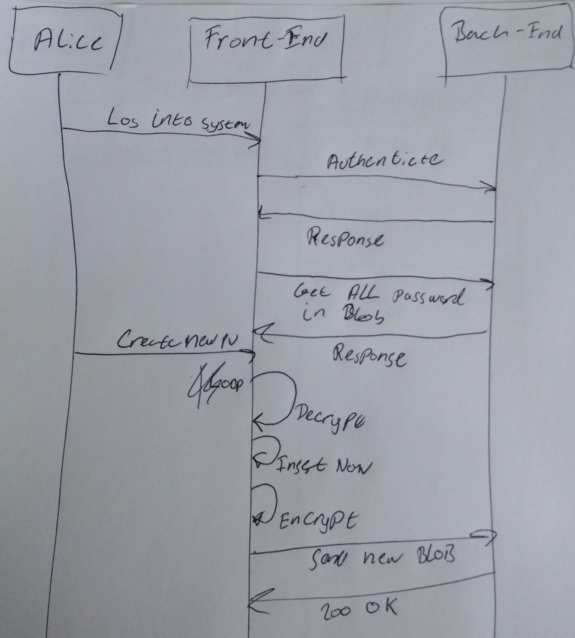
\includegraphics[width=\textwidth]{figures/design/sequence_blob_small.png}
				\caption{Squence diagram for creating new password using blob encryption.}
				\label{fig:seq_blob}
			\end{figure}

			The advantage of this, is that the blob practically can be encrypted with whichever scheme the user chooses: The back-end merely sends and receives blobs. However, it also has a \emph{major} drawback. This approach, unfortunately, results in large amounts of overhead: Every time a single entry is accessed, the entire blob needs to be decrypted. Same goes for updating: The entire blob will need to be both decrypted and encrypted again. While this might not be a huge issue with small datasets, it scales horribly for larger sets.

		\subsection{Per Entry Encryption}
			An alternative approach is that encryption could be employed on a per-entry basis. Using this scheme, some of the attributes per entry could then be encrypted. An example of such an entry could be a set consisting of a username, password, and URL. In this specific \emph{example} the password could be the only thing encrypted. 

			Using the same example before, of a password being added or updated, it is clear that encryption-wise, this solution is a lot more lightweight. \emph{Only} the updated / new fields are changed, leaving the remainder of the data unchanged. This sequence of events, is depicted on the sequence diagram on figure \ref{fig:seq_perentry} on page \pageref{fig:seq_perentry}. The drawback to this, is that additional information has the potential of being exposed in the database \emph{(unless the entire entry is encrypted)}.


			\begin{figure}[h!]
				\centering
				
\includegraphics[width=\textwidth]{figures/design/na.png}
				\caption{Squence diagram for creating new password using individual.}
				\label{fig:seq_perentry}
			\end{figure}

		\subsection{Sharing Is Caring}
			\label{sec:share}
			However, deciding the encryption scheme based on the previous sections is not possible. There is one important aspect, not yet considered: As stated in section \ref{sec:requirements} on page \pageref{sec:requirements} being able to share a password is a requirement. As such, it is important that a user, Alice, is able to share a password with another user, Bob -- and \emph{only} Bob.

			For this feature, an encryption scheme is needed which satisfies the following: Alice can share a single password with Bob, without Bob being able to access the remaining passwords. It should happen purely from Alice's part: No interaction with Bob should be necessary before a password is shared.


			\subsubsection{Proxy Re-Encryption}
				While the exact topic of \emph{password} sharing has not been sufficiently extensively covered in academic literature, topics as secured data sharing has. Since a shared password string is \emph{essentially} data, these techniques and approaches can also apply to this specific case. 

				A fairly new cryptographic concept used for data sharing is proxy re-encryption. A fair amount of academic literature exists on this topic, while \emph{actual} implementations are far more scarce. In ``POSTER: A Certificateless Proxy Re-Encryption Scheme for Cloud-based Data Sharing'' \cite{Wu:2011:PCP:2046707.2093514}, Wi, Xu, and Zhang describe their take on this encryption scheme for data sharing, which they call CL-PRE.

				While a complete analysis of their implementation is far beyond the scope of the current section, a brief overview of how it \emph{fundamentally} works, is seen on fig \ref{fig:sequence:cl-pre} on page \pageref{fig:sequence:cl-pre}.

				In this scenario three parties are involved: Alice, Bob, and a cloud. Both Alice and Bob has their own private/public-key set. Alice wishes to share a password with Bob. The data is encrypted with a symmetric data encryption key \emph{(DEK)}. The encrypted data is then sent to the cloud, alongside an access control list \emph{(ACL)}, a version of the DEK encrypted with Alice's public-key, and a re-encryption key. The re-encryption key is derived from Alice's private-key and Bob's public-key. When Bob requests access to the password, the cloud checks the ACL to see if he has access rights. If he has, the cloud uses a re-encryption algorithm, to transform the DEK into something which can be decrypted by Bob's private-key. Bob then downloads this data, and decrypts it locally using his key.

				%It is quite straight forward how proxy re-encryption could be used for this problem. Each password is encrypted using the DEK. The encrypted DEK is then stored alongside the password. As such, each password has their own unique DEK. When Alice wishes to share a password with Bob, she simply uploads the re-encryption key, derived from her private-key and Bob's public-key, for said password. Bob is then able to access the password. 

				Examining the scalability for this solution, it is shown that it \emph{could} be better. For each password a DEK needs to be stored -- no matter if the password is shared or not. While this is linear scaling, it still creates a fair amount of overhead.

				While this scheme inherently is \emph{everything} that is needed for this particular problem, one slight issue arises. First and foremost it is a recently new technology. This means that implementations are scarce at this point. While this shouldn't matter at this point in time -- since it is the \emph{design} of the solution being discussed -- it \emph{will} have ramifications down the road which needs to be considered. A general rule of thumb is to never ``roll your own'', when it comes to encryption. Existing libraries will have significant more exposure and will possibly have been through one or more security audits. This will most likely mean, that any implementation issues there might have been, should have been discovered and fixed.

				\begin{figure}[h!]
					\centering
					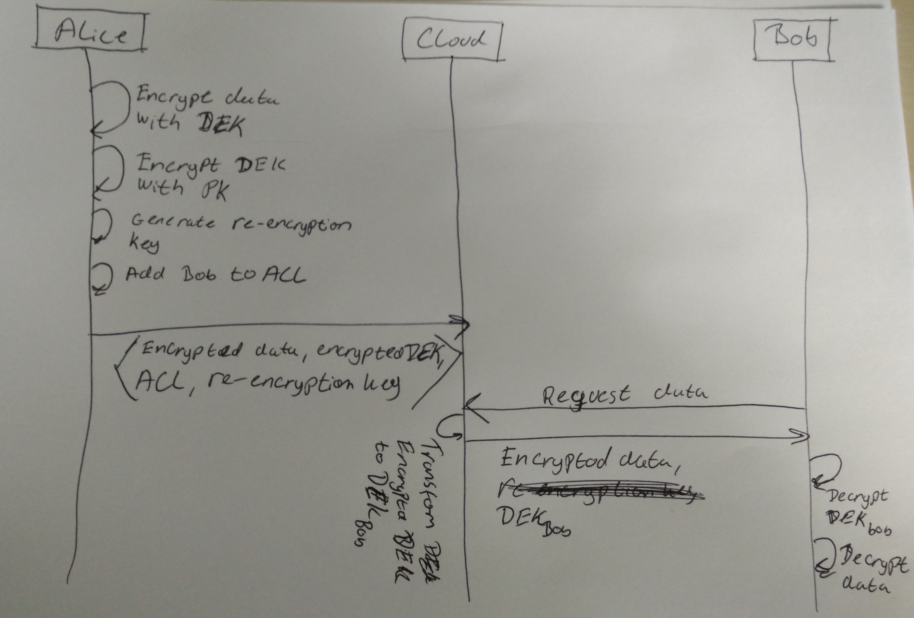
\includegraphics[width=\textwidth]{figures/design/sequence_cl-pre_small.png}
					\caption{Sequence diagram for sharing a password, using Wi, Xu, and Zhang's CL-PRE encryption scheme\cite{Wu:2011:PCP:2046707.2093514}.}
					\label{fig:sequence:cl-pre}
				\end{figure}

			\subsubsection{Pretty Good Privacy}
				While the previous section described a start-of-the-art, this approach is more classic. Pretty Good Privacy, or more commonly known simply as PGP, is a scheme dating back to the beginning of the 1990s. 

				PGP uses a combination of symmetric and asymmetric encryption. Whenever a chunk of data needs to be encrypted for sharing, a new symmetric key is generated. The symmetric key is used to encrypt the data. Afterwards, the symmetric key is encrypted using the recipients public-key. Then the encrypted data and the encrypted key is transmitted to the recipient, which can then decrypt the symmetric key, using his own private-key. 

				The reasoning behind this, is that symmetric encryption is \emph{several} magnitudes faster than asymmetric encryption. As such, it is \emph{far} more efficient to encrypt larger documents, using the symmetric key and \emph{then} encrypting said key, than directly encryption the document with an asymmetric key.

				%\textsc{..}
				Using this approach for the problem at hand is quite similar to the previous one. Each password has a unique symmetric encryption key, $SK$, which is never stored directly on the back-end. All users having access to said password, then has a copy of $SK$ encrypted with their own public-key stored. Sharing a password is then as simple as getting the recipients public-key, encrypting the $SK$ with said key, and uploading it to the server. The previous approach is depicted on figure \ref{fig:sequence:pgp} on page \pageref{fig:sequence:pgp}.

				One of the main arguments for using PGP is the fact that symmetric encryption is by far faster than asymmetric. However, in this case the plaintext is relatively small: A password most likely no longer than 72 characters. As such, the performance gained using PGP is pretty much gone. It would hardly take longer to encrypt such a password with asymmetric encryption, than it would for PGP to encrypt a symmetric key.

				Additionally, this solution has the same draw-back as proxy re-encryption. It requires that \emph{all} passwords have an symmetric key stored beside them. The same argument as before can be used again: While it in \emph{no} way can be considered ``bad'' scaling, it could be better.

				\begin{figure}[h!]
					\centering
					
\includegraphics[width=\textwidth]{figures/design/na.png}
					\caption{Squence diagram for sharing a password using the PGP scheme.}
					\label{fig:sequence:pgp}
				\end{figure}

			\subsubsection{Asymmetric Encryption}
				\label{sec:assymetric}
				A third option is to directly use asymmetric encryption. Each user has -- like previously -- a private and a public-key pair. Each password is then encrypted using the public-key and stored on the server. To access the password it simply has to be decrypted using the private-key. Sharing the password is simple as well. Simply fetch the public-key of the recipient, encrypt the password using said key, and upload the newly encrypted password. This is shown on figure \ref{fig:sequence:asymmetric} on page \pageref{fig:sequence:asymmetric}.

				One of strongest arguments for the PGP scheme, is that generally asymmetric encryption is significantly faster. However, since the plaintext would be rather small -- most likely below 100 bytes -- this problem is effectively null and void, leaving this scheme a \emph{viable} candidate.

				Using this approach is easily the most simple so far. Alice wishes to share a password with Bob. She fetches his public-key, encrypts the password with said key, and uploads the encrypted password to the back-end. Bob then merely needs to fetch the password and decrypt it, in a process virtually no different from when accessing his own passwords.

				As the astute reader might have figured out, this \emph{strictly} speaking isn't ``sharing'' a password. It is more of a ``sharing by cloning'' procedure. When the original password needs to be updated, it needs to be encrypted once per user it is shared to. This is \emph{definitely} a draw-back, compared to the previous solutions. From a storage perspective, however, this trumps the previous solutions. Storage wise, this is far more efficient than the previous solutions. When a password is shared, it is cloned and stored encrypted with the recipient's public-key, causing only an increased storage \emph{if} a password is shared.

				\begin{figure}[h!]
					\centering
					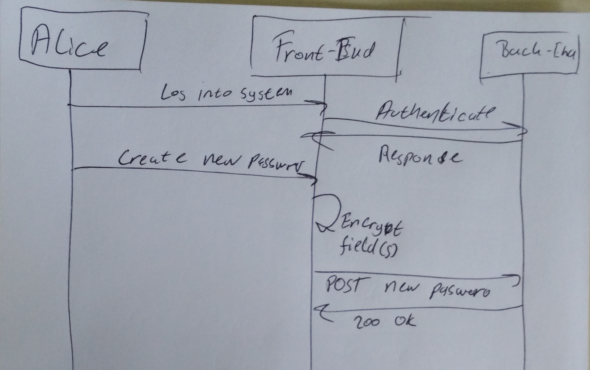
\includegraphics[width=\textwidth]{figures/design/sequence_perEntry_small.png}
					\caption{Squence diagram for sharing a password, when asymmetric encryption is used.}
					\label{fig:sequence:asymmetric}
				\end{figure}


				%Each user has both a private-key and a public-key stored on the server. When Alice wish to share a password with Bob, she requests the server for Bob's public-key. Once she gets this, she then re-encrypts the password with \emph{Bob's} public-key, and sends this to the server. This way, the password is never handles un-encrypted anywhere other than Alice's front-end. Finally, Bob can easily decrypt the password, using his own private-key. This sequence of events, is shown on figure \ref{fig:seq:assymetric} on page \pageref{fig:seq:assymetric}.

			\subsubsection{Making A Choice}
				\label{sec:encryption_choice}
				Having described three different approaches to solving the problem, it is time to decide exactly which should be used. All of them have their drawbacks -- all of them have their advantages. Since the asymmetric encryption approach has no acronym, it will be referred to as ``Asymmetric'' in the following tables.

				First and foremost, let us examine the availability of tools, cf. table \ref{table:comp:availability}. Admittedly, this should probably carry less weight in the design of the system, however, as mentioned earlier this \emph{will} effect the implementation heavily, should existing libraries not exist. While CL-PRE is just an example of a proxy re-encryption it is a general truth to these algorithms, that at this point in time they are more theoretical than practical -- unfortunately. In stark contrast to this, both PGP and asymmetric encryption algorithms have a plethora of implementations, for just about any combination of hardware and language available. As such, they're the clear favourites in this regard.

				\begin{table}
					\center
					\begin{tabular}{r|l}
						Solution 		& Available Implementations 	\\
						\hline
						CL-PRE 			& \red{Very Rare} 				\\
						PGP 			& \green{Several} 				\\
						Asymmetric 		& \green{Several} 				\\
					\end{tabular}
					\caption{Comparison of availability of implementations of the three encryption schemes.}
					\label{table:comp:availability}
				\end{table}

				Next, it is only fitting to compare the data requirements for these three approaches, cf. \ref{table:comp:data}. As was explained earlier, CL-PRE requires not only an encryption key stored alongside the password, but also a re-encryption key per user said password is shared to. Then there is PGP which only requires an extra encryption key \emph{per} user requiring access. Finally, there is the asymmetric approach which requires no extra data to be stored, due to it only using the users' private and public-keys. As such, the asymmetric approach is \emph{clearly} the favourite in this regard. 

				\begin{table}
					\center
					\begin{tabular}{r|l|l}
						Solution 		& Per Password Value  			& Per Share Value 	\\
						\hline
						CL-PRE 			& \red{Yes} 					& \red{Yes}			\\
						PGP 			& \green{No} 					& \red{Yes} 		\\
						Asymmetric 		& \green{No} 					& \green{No} 		\\
					\end{tabular}
					\caption{Comparison of data usage of the three encryption schemes.}
					\label{table:comp:data}
				\end{table}

				Finally, there is the matter of data processing, which is also an important aspect to take into account, cf. \ref{table:comp:data}. Creating a password with CL-PRE involves the following steps: First a symmetric DEK needs to be created, then the password is encrypted with said DEK, and finally the DEK is encrypted using the user's public-key. This totals to $3$ ``cryptographic steps''. PGP is essentially the same. First a new symmetric key is created, then the password is encrypted using that key, and finally the key is encrypted using the user's public-key. Hence, PGP also uses $3$ cryptographic steps. Using asymmetric encryption, however, only a single step is needed: Encrypt the password with the user's public-key.

				For creating a password, the asymmetric approach is clearly the favourite. Not only in the steps involved, but also just from its simplicity. However, this is not \emph{quite} the same when sharing a password. CL-PRE actually only needs a single step for updating a shared a password: Creating the re-encryption key. PGP on the other hand needs two operations: Decrypting the symmetric key, and re-encrypting it with the recipients public-key. Finally, there is the asymmetric approach. This approach needs $n$ operations, per update, where $n$ is the number of people the password is shared to. This \emph{huge} performance loss is due to the fact that it uses sharing by cloning. This is best illustrated with an example: If a password is shared with three people, it means that it exists four times in the back-end: Once encrypted with the owners public-key, and once with each of the people it is shared to. When the password is updated, it needs to be re-encrypted using \emph{each} of these peoples public-keys as well.

				In this case, it is \emph{quite} clear that the asymmetric approach is inferior, when $n$ is large. However, since this overall solution is based around individual password sharing, and not sharing between a group, it is fair to assume that $n$ will be low. As such, the performance loss significantly less than originally assumed.

				All of these three tables are combined into a single large table, on figure \ref{table:comp:complete_schemes} on page \pageref{table:comp:complete_schemes}. Looking at this table, it is quite clear that as long as the assumption of relative few shares per passwords hold, the asymmetric approach is the preferable one to use.

				\begin{table}
					\center
					\begin{tabular}{r|l|l}
						Solution 		& Creating A Password  	& Updating a Password 	\\
						\hline
						CL-PRE 			& \green{$3$} 					& \green{$1$}					\\
						PGP 			& \green{$3$} 					& \green{$2$} 					\\
						Asymmetric 		& \green{$1$}					& \red{$n$} 					\\
					\end{tabular}
					\caption{Comparison of cryptographic steps required for the three encryption schemes. $n$ represents the number of users a given password is shared to.}
					\label{table:comp:data}
				\end{table}

				\begin{table}
					\center
					\begin{tabular}{r|l|l|l|l|l}
						Solution 		& \rot{Available Implementations} & \rot{Storage Per Password Value}  	& \rot{Storage Per Share Value}	& \rot{Steps for Creating A Password} 	& \rot{Steps for Updating a Password} 	\\
						\hline
						CL-PRE 			& \red{Very Rare} 	& \red{Yes}		& \red{Yes} 	& \green{$3$} & \green{$1$} \\
						PGP 			& \green{Several} 	& \green{No}	& \red{Yes} 	& \green{$3$} & \green{$2$} \\
						Asymmetric 		& \green{Several} 	& \green{No}	& \green{No} 	& \green{$1$} & \yellow{$n$} \\
					\end{tabular}
					\caption{Complete comparison of the three schemes. $n$ represents the number of users a given password is shared to.}
					\label{table:comp:complete_schemes}
				\end{table}

		\subsection{Asymmetric Encryption Algorithm}
			Having decided on using the asymmetric approach, an algorithm for this needs to be decided. The two contenders for this algorithm is the RSA and ElGamal algorithm. Unfortunately, there does not seem to exist any \emph{sound} papers regarding their comparative strength and efficiency, and as such the choice must be based on something else.

			As such, it is chosen to go with RSA for the reason that its use is simply more widespread. Additionally, a keysize of $4096$ is chosen, as per the recommendations of European Union Agency for Network and Information Security \emph{(ENISA)}\cite[p.37]{enisa}.

			When using RSA, however, it is necessary to be aware of a vulnerability in using ``plain'' RSA. This vulnerability is described in \cite{boneh2000textbook} where an attack reducing the effective security to the half, is described. They also conclude that this can be avoided by using OAEP padding with RSA.

		\subsection{Key Management}
			\label{sec:keys}
			As the astute reader might have realized by now, there is a slight short-coming in what has previously been described. How the private and public-key is stored and transported is omitted \emph{(by choice)}. In an ideal world, all users would automatically have access to the rest of the users' public-keys, and their own private-key would be securely distributed to all devices. However, the world is far from ideal.

			Since the public-key is \emph{not} sensitive information. As such the easiest way to distribute these keys, is simply to store them on the server. This also makes it very easy for the client application to access these keys.

			However, that leaves the private-key. The most secure approach would probably be to let the user manage distributing this key themselves. However, this would end up being a very troublesome process and will lower the over-all user experience. Hence, an encryption scheme for storing the private-key on the server needs to be devised.

			\subsubsection{Choosing an Encryption Algorithm}
				While there exists a plethora of symmetric encryption algorithms, some are more used than others. These are the 3DES, Blowfish, and AES algorithms. As with any of these choices, there exists various pros and cons for each of the algorithms. 

				Several independent papers describe blowfish as the faster algorithm, quoting that since no known vulnerabilities exists for it, it is the best option for symmetric encryption\cite{thakur2011aes,singh2011comparison,verma2011peformance,ramesh2013performance}. While this might very well be true, one can not only compare these algorithms on efficiency, as security is as equally important -- if not more. 

				On the other hand the National Institute of Standards and Technology \emph{(NIST)} -- strictly speaking -- recommends the use of the 3DES and AES algorithms\cite{barker2012sp}, in their report for use of the 3DES algorithm they write:
				\begin{quote}
					\emph{Note: Through the year 2030, Triple DES (TDEA) and the FIPS 197 Advanced Encryption Standard (AES) will coexist as approved algorithms – thus, allowing for a gradual transition to AES. (The AES is another symmetric-based encryption standard approved by NIST.)}\\
					\cite{barker2012sp}
				\end{quote}
				On top of this, ENISA classifies Blowfish as a legacy algorithm, whereas AES is considered future proof\cite[p.20]{enisa}.

				As a consequence it is decided, that the AES algorithm will be used for protecting the private-key, stored on the server. While AES supports a number of different key sizes, AES-256 is chosen for the added security. Additionally, a random IV will need to be generated, due to how AES works.

			\subsubsection{Creating an Encryption Key}
				\label{sec:kdf}
				As with any encryption, AES-256 requires an encryption key. If the key is chosen to be stored on the server, this merely shifts the security risk -- it wont eliminate it. As such, the encryption needs to be based on something which is never stored on the server. The easiest, and by far most logical, way to achieve this, is to use a password. 

				But using a user's password as a asymmetric encryption key will \emph{not} result in enough entropy. Doing this will be \emph{very} insecure. alternatively an encryption key can be \emph{derived} from a password. This is a fairly common task, and is best performed using a so-called Key Derivation Function, or KDF for short. These KDF's are designed to be slow. Where regular hashing algorithms such as SHA-1 are designed to be fast and efficient, KDFs are designed to be exactly the opposite. This is done to slow down a possible brute-force attack against the hash. After all, the regular user will never be the wiser if hashing a single password takes $0.01$ seconds or $1$ seconds. But performing this calculating hundreds of thousands of times will add up, making the computational load for a bruteforce attack \emph{significantly} harder. 

				There exists a \emph{plethora} of various KDFs -- way too many to cover all of them in this section. However, the most widespread KDF is the PBKDF2 algorithm\cite{rfc2898}, which is developed by RSA Laboratories. However, in June 2015 the Password Hashing Competition was concluded\cite{phc}. The competition was held in an attempt to develop a new crypto standard for password hashing algorithms \emph{(practically the same as a KDF)}. Their recommendation is to use the Argon2 algorithm\cite{biryukov2015argon}. Based on this, The Open Web Application Security Project \emph{(OWASP)} made the following recommendation, in regards to password hashing:
				\begin{quote}
					\emph{Select:
						Argon2[*7] when it becomes available. Argon2 is the winner of the password hashing competition and should be considered as your first choice when solid implementations are available.
					}\\\cite{owasp_kdf}
				\end{quote}

				Since Argon2 is such a new algorithm, ``solid'' implementations might very well be difficult to find. But this project will adhere to OWASP's guidelines, as far as possible. As such, it is preferable if the project derives the symmetric encryption key using the Argon2 algorithm. As a final note, avoid multiple users having the same encryption key, a salt will need to be added as well. 

		\subsection{Comparison With Requirements}
			\label{requirement:fulfilled:sharing}
			\label{requirement:fulfilled:passwords_local}
			\label{requirement:fulfilled:encryption}
			Having decided that the solution will revolve around asymmetric encryption, using RSA keys of length 4096 which in return is secured by AES-256 encryption, it can be concluded that the solution fulfils the non-functional requirement \#\ref{requirement:encryption}:

			\vspace{-3ex}\begin{enumerate}
				\setlength\itemsep{0.1em}
				\setcounter{enumi}{4-1}
				\item Use encryption for storage should be viable for at least 5 years
			\end{enumerate}

			Furthermore, due to how the asymetric encryption is handled, not only can the users share passwords, but it can also be enforced, that a password is never even \emph{able} to be decrypted in the back-end. As such, it is concluded that the solution now fulfils the functional requirements \#\ref{requirement:sharing} and \#\ref{requirement:passwords_local}:
			\vspace{-3ex}\begin{enumerate}
				\setlength\itemsep{0.1em}
				\setcounter{enumi}{5-1}
				\item Password sharing
				\setcounter{enumi}{9-1}
				\item Passwords and private information should never be stored or handled unencrypted anywhere, other than the local device
			\end{enumerate}


			%As such, the checklist is updated which is reflected on figure \ref{tab:checklist_encryption} on page \pageref{tab:checklist_encryption}.

				%Having made choices regarding data encryption and protection, in the previous sections, it is now suitable to update the checklist found on figure \ref{tab:checklist_arch-comms} on page \pageref{tab:checklist_arch-comms}. Using the asymmetric approach and protecting the users' keys with a password derived symmetric key, it is clear that the following requirements are now fulfilled

	\section{Authentication}
		As with any program handling users' data, there need to be some sort of authentication method in place. Describing the authentication used for this project, will be split up into two categories: First it will be determined exactly how the API will be secured. Once this has been determined, it will be decided how to actually \emph{perform} this authentication.

		\subsection{Securing the API}
			There exists a number of different approaches for securing an API. These range from the built-in protocols in HTTP \emph{(HTTP Basic)} to more advanced enabling users to authenticate using their credentials from Google, for example \emph{(OAuth)}. One important aspect that needs to be stated first, is that this is a \emph{password manager}. Its sole purpose is to enable users to store \emph{strong} passwords to services such as Google. Hence, it would make little to no sense allowing a user to authenticating using their Google account. As such, a very fundamental decision is made here: The authentication scheme \emph{must} work with data stored on the back-end itself.

			\subsubsection{HTTP Basic}
				HTTP Basic is, as the name implies, the most basic form of authentication. It uses standard fields in the HTTP header, containing username and password for authentication purposes. Since it is intended to be a \emph{very} basic authentication method, the password is sent Base64 encoded. Since this is easily decoded, it is considered an extremely insecure protocol if used without HTTPS. Additionally, Basic is vulnerable to replay attacks, if used without HTTPS.

				If, however, combined with HTTPS the insecurity is some-what mitigated, as the password is no longer transmitted in cleartext \emph{(base64)}. However, despite some of the insecurities are mitigated, it still serves the issue that the client will have to store the username and password for usage, as it is needed to be sent with \emph{every} request.

			\subsubsection{HTTP Digest}
				HTTP Digest is another fairly fundamental approach to authenticating with a server, somewhat akin to Basic. Where Basic only Base64 encodes the password, Digest uses a combination of MD5 hashing and and a nonce to avoid replay attacks. 

			\subsubsection{Cookies}
				In the later history of websites, cookies have frequently been used for authentication purposes. Where Basic and Digest requires the credentials to be sent with each request, this approach only requires the so called cookie.

				When the user authenticates to the server, the server issues a cookie. This cookie contains a specific session id, which is also stored on the server. Whenever a request is made to the server, this cookie is then passed along with it. When the server receives said cookie, it checks its internal database and fetches any data relevant to said session. Traditionally cookies are used in combination with stateful websites, which is why it is often not used in RESTful APIs.

			\subsubsection{Tokens}
				Speaking in very general terms, tokens are somewhat similar to cookies: They're a little piece of code, stored in the browser. However, where as cookies are tied to a session on the server, tokens are not. Tokens merely represent a subject, or in this case a user. Upon receiving a request with a token attached, the server then checks the tokens validity and verifies that the subject has access to a given resource. These tokens are also often referred to as ``bearer tokens''.

				Where the previous possibilities pretty much only has a single option for each, tokens are a more diverse option. Generally there exist three primary versions of these tokens:
				\begin{itemize}
					\item Security Assertion Markup Language \emph{(SAML)}
					\item Simple Web Token \emph{(SWT)}
					\item JSON Web Token \emph{(JWT)}
				\end{itemize}
				Since the SAML specification requires the use of SOAP, this is disregarded in this context. The difference between SWT and JWT is that SWT can only be signed symmetrically using the HMAC algorithm, where as JWT \emph{also} supports asymmetric signing using an private/public keypair\cite{auth0_jwt}.

			\subsubsection{Making A Choice}
				While this aspect of the design might seem trivial to some, it is actually a very fundamental and important aspect: It defines how the front-end authenticates with the back-end. While any of the previous approaches are strictly speaking \emph{valid}, some are more obvious than others. The HTTP Digest, for instance, is almost unnecessary compared to the option of just running Basic over HTTPS, and \emph{of course} HTTPS is required.

				That leaves us with Basic, cookies and tokens. Since it has previously been established that it is beneficial for the back-end to be designed in such a way, that third party clients can connect to it, cookies are not optimal. Cookies are primarily intended for the browser and as such, would most likely end up being a hindrance if one should choose to develop a native client.

				As such it is down to Basic or tokens. Basic only has the option of sending the username and password in Base64, as covered earlier. Tokens, on the other hand have the option of sending an entire JSON payload. This opens the possibility for fine tuning the payload down the road and customizing it better to suit the implementation requirements. 

				Trusting the payload of the token requires a certain level of trust. Using symmetrical signing of the JWT for this purpose is \emph{not} suitable. However, using a keypair for signing the JWT \emph{ensures} that the token originated from the server, and not from the client. As such, a certain level of trust can be implied in the token.

				As such, it is chosen that the API will be secured using JWT tokens which will be signed by a private/public keypair.

		\subsection{Obtaining the Token}
			In the previous section it was decided that the API will be protected using JWTs. However, the process of obtaining said tokens were not discussed. There exists a number of different ways to obtain this.

			Anyone working within the industry will without a doubt have at least heard of OAuth and OAuth2. These two authentication protocols are used for users to authenticate to a service, without actually revealing their credentials to said service. Instead they reveal them to Google, for instance, which in return issues a token that is used for authenticating to the service. Earlier arguments were made for why these protocols are \emph{not} suited for this problem, however, certain derived protocols of these exists. Commonly they're known as 2-legged-OAuth and 2-legged-OAuth2. The reason to this is that there is only two actors involved: The user and the service. The OAuth provider, as they're called, are taken out of the equation. While this is definitely a valid option, it is deemed that it is simply too much overhead, for which is essentially a \emph{very} authentication purpose.

			A general consensus amongst professionals using these technologies \emph{(RESTful APIs and JWT tokens)} seem to be, that a simple endpoint expecting a HTTP body with a username and password field, is the way to go, as long as HTTPS is used\cite{jwt.io,auth0_jwt,tkalec}. As such, the same approach will be used for this project.

			Upon receiving the username and password from the user, the back-end compares the password against its database. If it is found to be a match, a new JWT is issued. The process of comparing and validating a user's password is elaborated in section \ref{sec:password}.

			\todo{CHAP and such is not needed, when SSL is enforced 100\%}

		\subsection{Password Storage \& Verification}
			\label{sec:password}
			In the previous section, the process of the server verifying the user's input password was treated as a sort of black box. In this section this process will be examined.

			Today, it is common knowledge that storing passwords in plain text is a \emph{huge} security risk. Salting and hashing passwords, is proper way to implement storage of passwords. However, when choosing a salting algorithm, it is important not to choose algorithms intended for checksums. Algorithms such as SHA-1 and SHA-256 are \emph{designed} to be fast. When trying to mitigate a bruteforce attack on a leaked database, this is \emph{not} desirable.

			As such, it is by far better to use a key stretching algorithm \emph{(or key derivation function)} which is intended to be slow. Since this \emph{exact} topic has already been covered by section \ref{sec:kdf} on page \pageref{sec:kdf}, the same conclusion is made:

			\begin{quote}
				\emph{Select:
					Argon2[*7] when it becomes available. Argon2 is the winner of the password hashing competition and should be considered as your first choice when solid implementations are available.
				}\\\cite{owasp_kdf}
			\end{quote}

		\subsection{Multi-Factor Authentication}
			\label{sec:mfa}
			In the past years there has become more and more focus on security. As a result of this, more and more people are using multi-factor authentication to ensure that access to their personal data is as ``safe'' as possible. 

			In the previous sections only single factor authentication was considered, however, as per the requirements, cf. section \ref{sec:requirements}, the solution will have to support two-factor authentication. All authentication forms fall under one of three categories:
			\begin{enumerate}
				\item Something you know
				\item Something you have
				\item Something you are
			\end{enumerate}
			Using a username and password combination, is falls under the category of ``something you know''. As such, an additional factor needs to be added. 

			In many of the existing systems, this ``extra'' factor of authentication usually falls under the category of ``something you have''. Physical one time passwords, text messages to your phone with a pin, or NemID \emph{(limited to Denmark)} all re-presents a physical entity which the user posses. This means that an attacker not only has to have guessed the user's password, but also have stolen the physical entity. This, in theory, makes it a lot safer.

			However, there are also pitfalls to using possession as an authentication requirement. First and foremost, it is required that the user has the entity available at all times. Without it, he or she can simply not authenticate any more. So in a case of theft, or simple loss, the user is effectively locked out of his or her account. While this definitely is a weakness to the approach, it is deemed that the gain of security highly outweighs the pitfalls.

			\subsubsection{Choosing the Second Factor}
				Using ``something you have'' as a second factor is by far the easiest additional security factor to add to an online system. This involves sending the user a one-time-password \emph{(OTP)}. Some companies do this by providing physical tokens and some by developing their own internal system and accompanying app \emph{(Blizzard Entertainment, for instance)}. While this definitely is an option, it is also by far the most expensive. Dedicated hardware needs to be manufactured, or a separate application needs to be developed. Other companies choose to use text messages as a way of delivering one-time-passwords. The disadvantage to this approach is that a SMS gateway is required.

				A far more universal -- and partially plug'n'play -- approach exists, in the two most common OTP algorithms: HMAC-Based One-Time Password Algorithm\cite{rfc4226}, commonly known as HOTP, and Time-Based One-Time Password Algorithm\cite{rfc6238}, commonly known as TOTP. 

				\textbf{HOTP}\\
				HOTP requires to values to work. First and foremost there is a secret, which is shared behind the HOTP client and the back-end. Secondly, both -- separately -- manages a counter of how many times a OTP has been used. Using these two variables and the HMAC hashing algorithm, the OTP is then calculated. 

				\textbf{TOTP}\\
				TOTP, by many thought to be the successor to HOTP, is roughly the same as HOTP, except it uses a value derived from a timestamp, instead of a counter. The value is derived based on two variables, $X$ and $T0$, where $T0$ is a Unix timestamp from when counting starts, and $X$ is the interval the key is valid for. Usually $T0$ is set to $0$, which is the Unix epoch and $X$ is set to $30$ seconds. The value is then calculated as $T = (now - T0)/X$, cf. \cite[Sec. 4.2]{rfc6238}.

				Both have their respective advantages and disadvantages. The advantage of HOTP is that it is independent from the system clock of the two devices, which is known to drift from time to time. The disadvantage, however, is that the counter needs to be synchronized between the client and the back-end. If the user generates OTPs without using them, they cease to be synchronized. To fix this, they back-end must initiate what the RFC defines as the ``resynch protocol'', which will result in the counter being updated in the back-end. Another drawback is that HOTP requires a counter to be stored in the back-end.

				The advantage of TOTP is that OTPs are generated contentiously. Where the HOTP key lives for a lot longer \emph{(indefinitely)} the TOTP only has a certain window of validity. Common configurations of TOTP lets keys validate for plus/minus two minutes, to account for time drift between the client and the back-end. This, however, is also the weakness of TOTP: Time drift. If the client and the back-end does not operate with the same current time, the OTP will simply not validate.

				Taking the pros and cons into consideration, it is chosen that the TOTP algorithm will be supported in this solution. It is believed that the only inherent draw-back in the algorithm, is mitigated for the most part, by modern systems being fairly good at making sure their internal time is correct.

		\subsection{Comparison With The Requirements}
			\label{requirement:fulfilled:auth}
			\label{requirement:fulfilled:change}
			\label{requirement:fulfilled:two-factor}
			In the previous sections, the various options for securing the API was covered, and it was chosen to use JWT tokens. Additionally, the process of obtaining the token was discussed. Since HTTPS is enforced, a simple API endpoint with the username and password as payload will work quite nicely. It was also decided, that the passwords will be hashed using the Argon2 algorithm, if a decent implementation is available. Otherwise, another key derivation function will be used, in accordance with OWASP's recommendations. As such, it is concluded that the solution fulfil the functional requirements \#\ref{requirement:auth} and \#\ref{requirement:change}:

			\vspace{-3ex}\begin{enumerate}
				\setlength\itemsep{0.1em}
				\setcounter{enumi}{14-1}
				\item Allow user authentication based on a single master password, per user
				\item Allow the user to change his or her master password
			\end{enumerate}

			Additionally, it was decided that the solution will support \emph{optional} TOTP two-factor authentication. As such, it is concluded that the solution also fulfils the functional requirement \#\ref{requirement:two-factor}:
			\vspace{-3ex}\begin{enumerate}
				\setlength\itemsep{0.1em}
				\setcounter{enumi}{16-1}
				\item Support two-factor authentication
			\end{enumerate}

	\section{Attaining Pseudo-Zero-Knowledge}
		As per the requirements it is known that the passwords must never be stored or handled unencrypted on the server. Previously, as an extension of this, it has been argued that letting the back-end as much as having the \emph{ability} of decrypting the stored passwords is ill advised. Hence, there should be no way of inferring the user's password for storing their private-key \emph{(see \ref{sec:encryption_choice} on page \pageref{sec:encryption_choice})} from \emph{anything} stored in the back-end.

		As the reader might have realized by now, \emph{two} passwords are -- unfortunately -- needed. One password for authentication purposes, and one for decrypting the private-key. From now on, these two passwords are known as the authentication password and the decryption password.
 
		The authentication password is the one which is stored on the server, in its salted and hashed form \emph{(see \ref{sec:password} on page \pageref{sec:password})}. This is sent -- in clear text -- to the server for verification purposes. The decryption password is used -- with a salt -- to derive the symmetric encryption key used for the client to decrypt the private-key \emph{(see \ref{sec:keys} on page \pageref{sec:keys})}. At no point in time will the front- or back-end attempt to compare these two passwords, however, it is \emph{strongly} recommended that they be different. As long as they are different it effectively ensures that the back-end can \emph{not} infer the correct decryption key, and as such can never actually inspect the passwords stored on it. This property is dubbed Pseudo-Zero-Knowledge.

		\subsection{Comparison With the Requirements}
			While this feature does not fulfil a requirement directly, it goes to strengthen the way that the requirement regarding un-encrypted data is handled.

	\section{User Hierarchy \& Creation}
		\label{sec:user:diff}
		As with any system, certain functionality should not be exposed to the regular users. As such, user differentiation is needed. There are two different schools of thought when it comes to this: The simple approach and the sophisticated approach.

		The simple approach involved simply storing a boolean value, indicating whether or not the user is an admin or not. While this solution is \emph{very} simple and is most likely the easiest to implement, it has its drawback: There are only two user levels. If one, later down the road, then wanted to add a third user level, this would require large amounts of refactorisation in the code.

		The more sophisticated approach is creating a user hierarchy. This hierarchy would then only consist of two users in the beginning: User and Admin. Based on this hierarchy the solution could enable and disable various aspects based on a user's level. The benefit of this approach, is that later on, several new levels could be added in between the User and the Admin, with varying privileges. How this is stored in the database is up to the implementation, but something as simple as an integer could be sufficient for storing this.

		Since the functionality that needs to be kept away from the regular user, is nothing more than some administrative functionalities here and there, it can be argued that there never will be a need for more user levels. As such, it is chosen to go with the simple approach. 

		Exactly how this user differentiation will be used, will be discussed in the following sections.

		\subsection{Creating Users}	
			Normally, in a solution like the one being designed here, creating the user would be a simple HTTP POST containing the user information. However, since this system will be run by individuals, the owner needs control over exactly \emph{which} users are being created. Hence, open registration is not desirable.

			As such, creating a user will need an ``invite'' of sorts. These invites can then be consumed, in order to create a new user. The most straight forward approach is to let the invite ID simply be the database's auto-incremented ID. However, this might not be a good idea. As most database systems utilize auto-incremented IDs, it would be possibly for an attacker to guess the next ID. As such, the token used needs to be non-sequentially generated.

			The easiest way to do this, is to simply generate a new Universally Unique Identifier \emph{(UUID)} for each invite generated. The UUID is then the token used for accepting an invite. Doing it this way, prevents anyone from guessing the ID of the invite issued next. Putting a lifespan on the invite likewise mitigates a guessing attack, in case of unused invites. For practicalities sake the lifespan will be set to 24 hours.

		\subsection{Creating the First User}
			As was decided in the previous section a user can only be created by an invite issued by an admin. However, when the system is first initalized, the user database would be empty, and there exists no admin who can issue an invite.

			As such, during the initialization process, an admin user will \emph{have} to be created. Using the industry standard, the username and password of this first account will be:
			\begin{verbatim}
				Username:      admin
				Password:      admin
			\end{verbatim}
			Upon first login, the user will then have to be prompted to change not only the password, but also the username, for security purposes.

		\subsection{Breaking the REST Principles On Purpose}
			While one of the pillars of REST APIs is that it should be stateless, sometimes this is just not feasible. One example of this, is when enabling two-factor-authentication for users. The back-end \emph{should} verify that the user has gotten the correct secret \emph{(see \ref{sec:mfa} on page \pageref{sec:mfa})}, before actually storing the secret in the database and enabling two-factor authentication. 

			If this verification is not done, the solution will be susceptible to the following scenario, resulting in a user being locked out:
			\begin{enumerate}
				\item User requests to enable 2-Factor-Authentication \emph{(2FA)}
				\item Back-end generates 2FA secret, sends it to user, and stores it
				\item User does not receive correct secret, or forgets to save it, or some other scenario where the secret is not stored correctly
				\item User logs out
				\item User attempts to log in, using the wrong secret
			\end{enumerate}

			As such, a verification step \emph{(which is commonly seen)} is required. This can be easily achieved by having the solution store a cached map, between user ID and the 2FA secret. When a new secret is generated, it is deposited in this cache, instead of the database. A specific API endpoint then exists, for verifying this secret. The verification process is exactly the same process which would be used for logging in. Once the cached secret is verified against the received token, the secret is stored in the database and 2FA is enabled for the user.

			While it is recognized that this violates essential principles of REST, it is deemed \emph{necessary} to do so.


		\subsection{Comparing with the Requirements}
			\label{requirement:fulfilled:multi_user}
			\label{requirement:fulfilled:admin_user}
			\label{requirement:fulfilled:add}
			In the previous sections it has been established how the system will differentiate between admins and users, and now invites will work. As such, it is concluded that the solution fulfil the functional requirements \#\ref{requirement:multi_user}, \#\ref{requirement:admin_user}, and \#\ref{requirement:add}:

			\vspace{-3ex}\begin{enumerate}
				\setlength\itemsep{0.1em}
				\setcounter{enumi}{2-1}
				\item Multi-user support
				\item Support differentiating between admin users and regular users
				\setcounter{enumi}{6-1}
				\item Only admin can add a user -- or invite a user -- to the solution
			\end{enumerate}

	\section{Auditing of Access}
		\label{sec:audit}
		Since it is peoples passwords being handled, some sort of audit log is preferable. Simply put, an audit log contains entries of when certain actions took place. For instance, it could be whenever a user authenticates the service, an audit log entry -- or simply entry -- is generated. Later on, the user can review these entries. This way, the user can easily see if an authentication has taken place, somewhere that he or she was not.

		When creating an audit log, it is very tempting to simply create an entry for \emph{everything}. However, while this will contain the data the user would need, it will be \emph{too} much data. Not only for the user to review, but also for the back-end to store. As such, first and foremost, it is necessary to determine exactly which events are necessary to log.

		Obviously, there is the matter of authentication. Both successful and failed authentication attempts will have to be logged. With this information, a user can quickly determine if access has been made from a device which he or she has not used. Furthermore, access to passwords should be logged. This access can call into any of four categories of actions: Create, read, update, and delete. These actions also apply to shared passwords. While the create actions could be used to denote a newly shared password, for the sake of usability a Share action is used instead. The remaining actions, read, update, and delete, also applies to shared passwords. As such, it is concluded that there will be \emph{seven} actions:
		\begin{enumerate}
			\item Success
			\item Failure
			\item Share
			\item Create
			\item Read
			\item Update
			\item Delete
		\end{enumerate}

		\begin{table}
			\begin{tabular}{r | c | c | c }
							& \textbf{Authentication} 		& \textbf{Passwords} 		& \textbf{Shared Passwords} 	\\
				\hline
				Success 	& \cmark 						& \xmark 					& \xmark 						\\
				Failure 	& \cmark 						& \xmark 					& \xmark 						\\
				Share 		& \xmark 						& \xmark 					& \cmark 						\\
				Create 		& \xmark 						& \cmark 					& \xmark 						\\
				Read 		& \xmark 						& \cmark 					& \cmark 						\\
				Update 		& \xmark 						& \cmark 					& \cmark 						\\
				Delete 		& \xmark 						& \cmark 					& \cmark 						\\
			\end{tabular}
			\caption{Which targets the various actions describe}
			\label{table:actions}
		\end{table}

		Each of these actions apply to either authentication \emph{(1 \& 2)} or passwords \emph{(3-7)} and shared passwords \emph{(2 \& 4-7)}. This relation is also shown on figure \ref{table:actions} on page \pageref{table:actions}.
		
		However, this information is hardly enough, to properly audit the entries. As such, information such as the timestamp for the event and the hostname of the machine, will greatly aid in the process of auditing. 

		\subsection{Comparison With Requirements}
			\label{requirement:fulfilled:audit}
			Having decided on what data should be logged for audit, it is concluded that the solution now fulfil the functional requirement \#\ref{requiremen:audit}:
			\vspace{-3ex}\begin{enumerate}
				\setlength\itemsep{0.1em}
				\setcounter{enumi}{13-1}
				\item Extensive auditing
			\end{enumerate}

	\section{Modelling the System}
		\label{sec:modelling}
		In the previous sections, all of the various requirements have been thoroughly discussed. In this section, all of these requirements will be condensed into the actual models used, in the system. 

		\subsection{The User Model}
			The User model is the most basic structure in the project. It represents -- obviously -- each individual user. As such, three very basic attributes need to be present: Username, password, and salt. The username will appear in cleartext, and the password and salt are the results of the hashing algorithm and is most likely in hexadecimal format. While some hashing functions store the generated salt in the resulting password hash, some do not. As such it has been deemed beneficial to have an dedicated variable for this. Next, in section \ref{sec:user:diff} on page \pageref{sec:user:diff} it was determined that user and admin differentiation would be done using a simple boolean and for this purpose a field called isAdmin is added.

			In sections \ref{sec:encryption_choice} and \ref{sec:kdf} on pages \pageref{sec:encryption_choice} and \pageref{sec:kdf}, respectively, it was determined that asymmetric encryption will be used. As such, a private-key and a public-key will need to be stored, additionally it was determined that a salt and IV needs to be stored. 

			Finally, as per section \ref{sec:mfa} on page \pageref{sec:mfa}, there a 2FA secret will need to be stored. Furthermore, a boolean toggle value determining whether or not 2FA is enabled for said user, is stored as well.

			As such, the final User model contains the fields listed on table \ref{fig:model:user} on page \pageref{fig:model:user}.

			\begin{table}[p]
				\centering
				\begin{tabular}{r|l}
					\textbf{Attribute} 		& \textbf{Type} 		\\
					ID 						& Unknown 	\\
					username 				& String 	\\
					password 				& String 	\\
					salt 					& String 	\\
					isAdmin 				& Boolean 	\\
					privateKey  			& String 	\\
					publicKey 				& String 	\\
					IV 						& String 	\\
					privateKeySalt 			& String 	\\
				\end{tabular}
				\caption{Fields of the User model}
				\label{fig:model:user}
			\end{table}

		\subsection{The Category Model}
			\label{sec:model:category}
			Before delving into the core model, the Password model \emph{(see the following section)} it is required to cover an auxiliary model: The Category. Since it has already been determined that it is required for the solution to structure passwords in multiple levels, a data structure for this is required.

			First and foremost, it is important to realise that the classical ``folder'' structure, is nothing more than what is commonly known as a tree. Trees consists of internal nodes and leafs. Nodes have children. These children can be other nodes, or a leaf. A leaf is a final child -- it is last element in the branch. An example of such a tree is seen on figure \ref{fig:example:tree} on page \pageref{fig:example:tree}.

			This structure can be translated very easily to the structure needed for password organization. The root and the internal nodes represent the various categories, and the leafs represent the passwords. As such, it will look like figure \ref{fig:example:passwordtree} on page \pageref{fig:example:passwordtree}.

			Multiple data structures exist to solve this exact problem. The simplest of them all, is the adjacency list. In this approach, each element simply stores a reference to either its parent or its children \emph{(top-down or bottom-up)}, depending on the implementation. This allows for the structure to be stored ``flat'', i.e. in a table, or an array, and when required the actual tree can be built from the data. Examples of these notations are found on tables \ref{table:example:tree:buttomup} and \ref{table:example:tree:topdown} on pages \pageref{table:example:tree:buttomup} and \pageref{table:example:tree:topdown}, respectively. The examples are based on the tree structure from figure \ref{fig:example:passwordtree} on page \pageref{fig:example:passwordtree}.

			While this approach might inherently be slower than other algorithms, cf. \cite{heirarchial_database}, it is believed that due to the relatively small datasets -- which is \emph{assumed} to be used -- it will have little effect. As such, the simplicity of the storage scheme a makes it perfect for this use.

			\begin{table}[p]
				\centering
				\begin{tabular}{c|c|c}
					\textbf{ID} 	& 	\textbf{Name} 	& \textbf{Parent} 	\\
					\hline
					\hline
					1 				& Root 				& Null 				\\
					2 				& Category1 		& 1 				\\
					3 				& Category2 		& 1 				\\
					4 				& Category1.1 		& 2 				\\
					5 				& Category1.2 		& 2 				\\
				\end{tabular}
				\caption{Flat tree structure, using bottom-up adjacency}
				\label{table:example:tree:buttomup}
			\end{table}
			\begin{table}[p]
				\centering
				\begin{tabular}{c|c|c}
					\textbf{ID} 	& 	\textbf{Name} 	& \textbf{Children} \\
					\hline
					\hline
					1 				& Root 				& [1,2] 			\\
					2 				& Category1 		& [4,5] 			\\
					3 				& Category2 		& [] 				\\
					4 				& Category1.1 		& [] 				\\
					5 				& Category1.2 		& [] 				\\
				\end{tabular}
				\caption{Flat tree structure, using bottom-up adjacency}
				\label{table:example:tree:topdown}
			\end{table}

			\begin{figure}[h!]
				\centering
				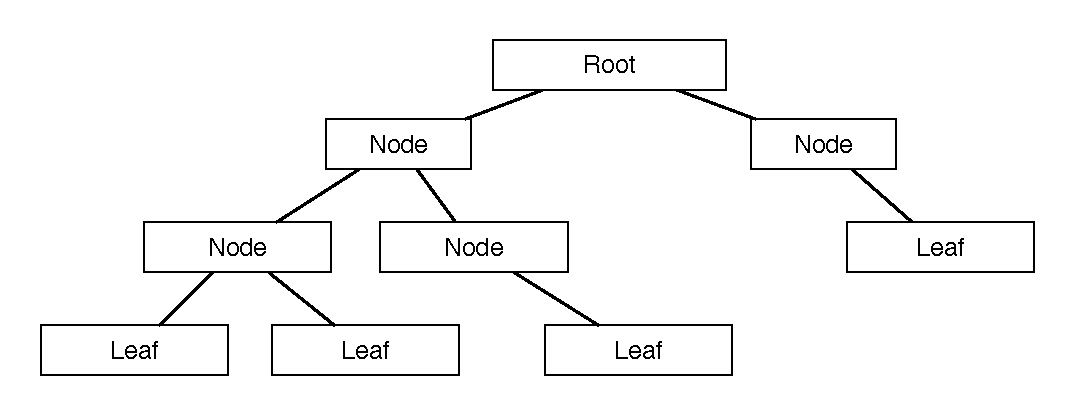
\includegraphics[width=\textwidth]{figures/design/uml/generic-tree.eps}
				\caption{Example of a tree.}
				\label{fig:example:tree}
			\end{figure}
		
			\begin{figure}[p]
				\centering
				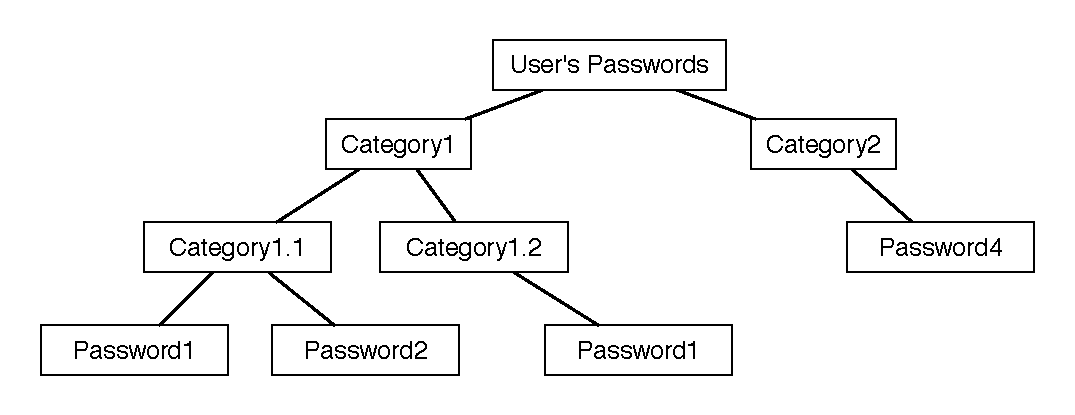
\includegraphics[width=\textwidth]{figures/design/uml/password-tree.eps}
				\caption{Example password structure in a tree.}
				\label{fig:example:passwordtree}
			\end{figure}

			As such, it is determined that the Category model will contain the fields listed on table \ref{fig:model:category} on page \pageref{fig:model:category}. On figure \ref{fig:relationship:category-user} on page \pageref{fig:relationship:category-user}, the relationship between the Category model and the User model is depicted, as well as the recursive definition of structure with itself.


			\begin{table}[p]
				\centering
				\begin{tabular}{c|c}
					\textbf{Attribute} 		& \textbf{Type} 		\\
					ID 						& Unknown 	\\
					title 					& String 	\\
					owner 					& User ID 	\\
					Parent / Children List 	& Parent ID / List of Children IDs 	\\
				\end{tabular}
				\caption{Fields of the Category model}
				\label{fig:model:category}
			\end{table}
			\begin{figure}[p]
				\centering
				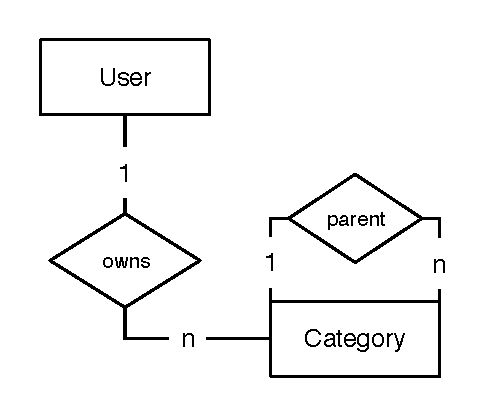
\includegraphics[scale=0.75]{figures/design/uml/user-category-relation.eps}
				\caption{The Category models relationship with the User model.}
				\label{fig:relationship:category-user}
			\end{figure}

			%\subsubsection{Algorithm: Generating the Structure}

			%\subsubsection{Algorithm: Deleting a Category}

		\subsection{The Password Model}
			\label{sec:model:model}
			Having described the Category model fully, the Password model can now correctly be explained. First and foremost it will consist of the fields that generally make up a password entry: A title, a username, a password, an URL, and a note. However, the passwords needs a way to connect with a user. For this purpose, a reference to the User models ID is needed. This reference is known as owner, i.e. the user who owns the password. Finally, to achieve the structure, as described in the previous section, a password is a child of a category. Hence, the Password model will need a reference to a parent Category's ID. These references are also depicted on figure \ref{fig:relationship:password} on page \pageref{fig:relationship:password}.

			As such, the final Password model contains the fields listed on table \ref{fig:model:password} on page \pageref{fig:model:password}.

			\begin{table}[p]
				\centering
				\begin{tabular}{c|c}
					\textbf{Attribute} 		& \textbf{Type} 	\\
					ID 						& Unknown 			\\
					title 					& String 			\\
					username 				& String 			\\
					password 				& String 			\\
					url						& Boolean 			\\
					note  					& String 			\\
					owner 					& User ID 			\\
					parent 					& Category ID 		\\
				\end{tabular}
				\caption{Fields of the Password model}
				\label{fig:model:password}
			\end{table}
			
			\begin{figure}[p]
				\centering
				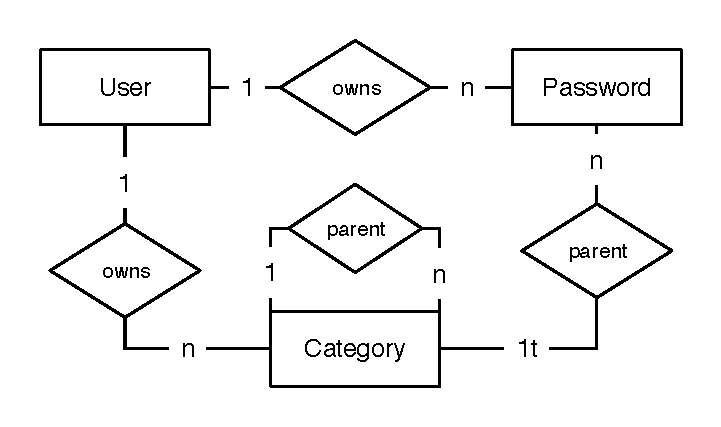
\includegraphics[scale=0.75]{figures/design/uml/user-password-category-erd.eps}
				\caption{A Password's connections to the User and Category models.}
				\label{fig:relationship:password}
			\end{figure}

		\subsection{The Shared Password Model}
			Having decided that the password sharing mechanism will be sharing by cloning, 

			Sharing a password can be achieved easily, by simply storing a reference to a user's password, under the ownership of another user. As such, each shared password entry will contain a reference to the original password. Using this reference, fields such as the username etc., can easily be obtained. However, since the \emph{actual} password is encrypted using each users individual key, this needs to be stored as well. To let the user receiving the shared password organize it as he or she sees fit, a reference to a Category ID is needed. Finally, references to the original owner and password, will make certain operations a lot easier. These relations are all shown on figure \ref{fig:relationship:sharedpassword} on page \pageref{fig:relationship:sharedpassword}, albeit the internal relations between User, Password, and Category has been omitted for clarity.

			As such, it is determined that the Shared Password model will contain the fields listed on table \ref{fig:model:sharedpassword} on page \pageref{fig:model:sharedpassword}. 

			\begin{table}[p]
				\centering
				\begin{tabular}{c|c}
					\textbf{Attribute} 		& \textbf{Type} 		\\
					ID 						& Unknown 		\\
					owner 					& User ID \\
					originOwner 			& User ID \\
					parent 					& Category ID \\
					password 				& String \emph{(Base64 Encoded)} \\
					originPassword 			& Password ID 		\\
				\end{tabular}
				\caption{Fields of the Password model}
				\label{fig:model:sharedpassword}
			\end{table}

			An example such an entry could be the following. Two users exists, as seen on table \ref{fig:example:sharedpassword:users} on page \pageref{fig:example:sharedpassword:users}, Alice and Bob \emph{(irrelevant user data has on purpose been left out)}. Alice owns a password with the title ``SamplePassword'', the details of which are shown on table \ref{fig:example:sharedpassword:samplepassword} on page \pageref{fig:example:sharedpassword:samplepassword}. Alice now wishes to share this password with Bob. As such, an entry is created, containing the information found on figure \ref{fig:example:sharedpassword:sampleshare} on page \pageref{fig:example:sharedpassword:sampleshare}.
			\begin{table}[p]
				\centering
				\begin{tabular}{r|l}
					\textbf{ID} 		& \textbf{Username} \\
					42 					& Alice 			\\
					1337  				& Bob 				\\
				\end{tabular}
				\caption{Sample user data}
				\label{fig:example:sharedpassword:users}
			\end{table}

			\begin{table}[p]
				\centering
				\begin{tabular}{c|c}
					\textbf{Attribute} 		& \textbf{Type} 											\\
					ID 						& 127 														\\
					title 					& SamplePassword 											\\
					username 				& SampleUser 												\\
					password 				& QmFzZTY0IEVuY29kZWQgUGFzc3dvcmQ= 							\\
					url						& www.some.com 												\\
					note  					& This is a sample password 								\\
					owner 					& User ID 													\\
					parent 					& Category ID 												\\
				\end{tabular}
				\caption{Sample password owned by Alice}
				\label{fig:example:sharedpassword:samplepassword}
			\end{table}

			\begin{table}[p]
				\centering
				\begin{tabular}{c|c}
					\textbf{Attribute} 		& \textbf{Type} 											\\
					ID 						& 666 														\\
					owner 					& 1337 														\\
					originOwner 			& 42 														\\
					parent 					& null 														\\
					originPassword			& 127 														\\
					password				& QmFzZTY0IEVOQ09ERUQgUGFzc3dvcmQ= 							\\
				\end{tabular}
				\caption{Sample of a shared password, shared from Alice to Bob.}
				\label{fig:example:sharedpassword:sampleshare}
			\end{table}

			\begin{figure}[p]
				\centering
				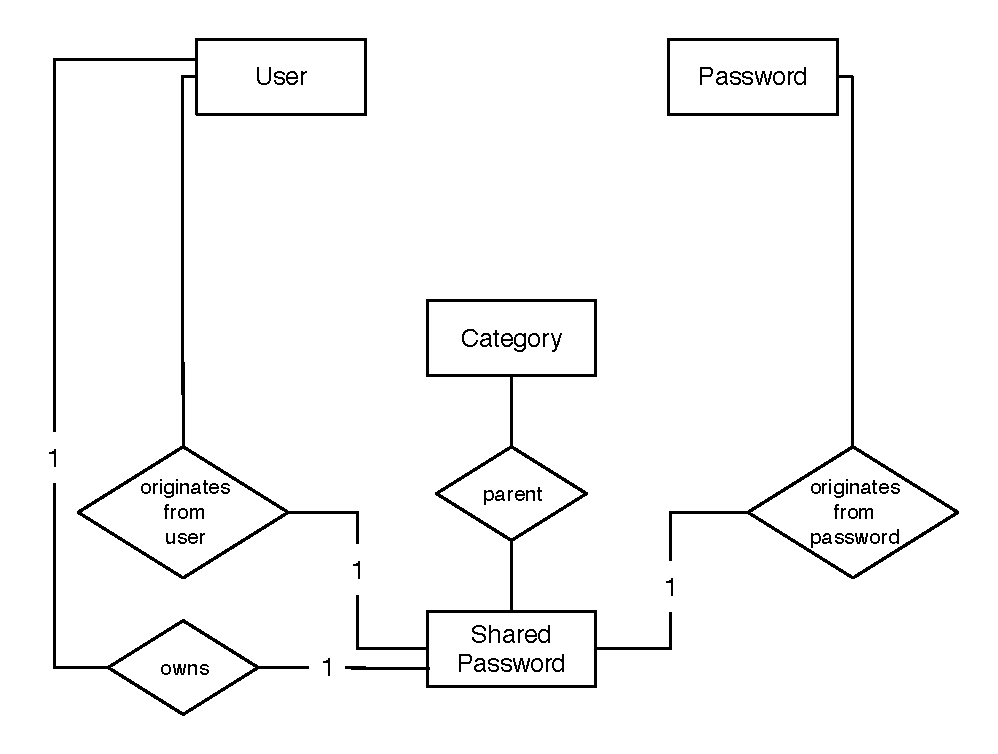
\includegraphics[scale=0.75]{figures/design/uml/sharedpassword-ER-diag.eps}
				\caption{Shared Password's connections to the User, Password, and Category models.}
				\label{fig:relationship:sharedpassword}
			\end{figure}

		\subsection{The Invite Model}
			While the previous models have been very intertwined, the Invite model stands apart by quite a lot simpler. As has already been determined, the Invite model will need a UUID. Since this will, in the end, be part of an invite URL, this field is simply called the link. Furthermore, an expiration date will need to be stored, as it has been determined that the invite will only be valid, for 24 hours. As such, this \emph{very} simple model determined to contain the fields listed on table \ref{fig:model:invite} on page \pageref{fig:model:invite}. 
			
			\begin{table}[p]
				\centering
				\begin{tabular}{c|c}
					\textbf{Attribute} 		& \textbf{Type} 		\\
					ID 						& Unknown 		\\
					link  					& UUID \\
					expires 				& Unix timestamp \\
				\end{tabular}
				\caption{Fields of the Password model}
				\label{fig:model:invite}
			\end{table}

		\subsection{The Audit Model}
			Finally, there is the audit model. As described in section \ref{sec:audit} on page \pageref{sec:audit}, each entry should contain one of six actions. While this could easily be achieved using an enum, not all database technologies support this data structure. As such, an integer mapping is used. In practice, this means that each action is translated to an integer, before being stored. When retrieved, the same integer is used to generate the actual name of the action. This mapping is shown on figure \ref{table:audit:actionmapping} on page \pageref{table:audit:actionmapping}.

			What is a challenge when modelling these audit entries, is the reference to one of three things: Authentication attempts, passwords and shared passwords. Because it is a reference to multiple fields \emph{(the entry's target)}, a traditional database foreign key reference is simply not possible. As such, the reference will need to be stored in an integer \emph{(unfortunately loosing any restrictions from the relations, in the process)}. However, it is still needed to differentiate between an ID for a Password and for a Shared Password. As such, the targets type will need to be stored as well. Finally, as was decided previously, a hostname and a timestamp will need to be stored as well.

			\begin{table}[h!]
				\centering
				\begin{tabular}{r | l}
					\textbf{Action} 	& \textbf{Integer} 	\\
					\hline
					Create 				& 0 				\\
					Read 				& 1 				\\
					Update 				& 2 				\\
					Delete 				& 3 				\\
					Share 				& 4 				\\
					Success 			& 5 				\\
					Failure 			& 6 				\\					
				\end{tabular}
				\caption{Integer mapping of audit actions.}
				\label{table:audit:actionmapping}
			\end{table}

			\begin{table}[p]
				\centering
				\begin{tabular}{r|l}
					\textbf{Attribute} 		& \textbf{Type} 		\\
					ID 						& Unknown 	\\
					userId 					& User ID 	\\
					targetType 				& String 	\\
					targetId				& Integer 	\\
					action					& Integer 	\\
					time  					& Datetime 	\\
					host  					& String 	\\
				\end{tabular}
				\caption{Fields of the Audit model}
				\label{fig:model:audit}
			\end{table}

			As such, it is determined that the Audit model will contain the fields listed on table \ref{fig:model:audit} on page \pageref{fig:model:audit}. On figure \ref{fig:relationship:audit-user} on page \pageref{fig:relationship:audit-user}, the relationship between the Audit model and the Password and Shared Password models are depicted, with adjusted syntax to meet the slightly unique approach required for this model to work.
			
			\begin{figure}[p]
				\centering
				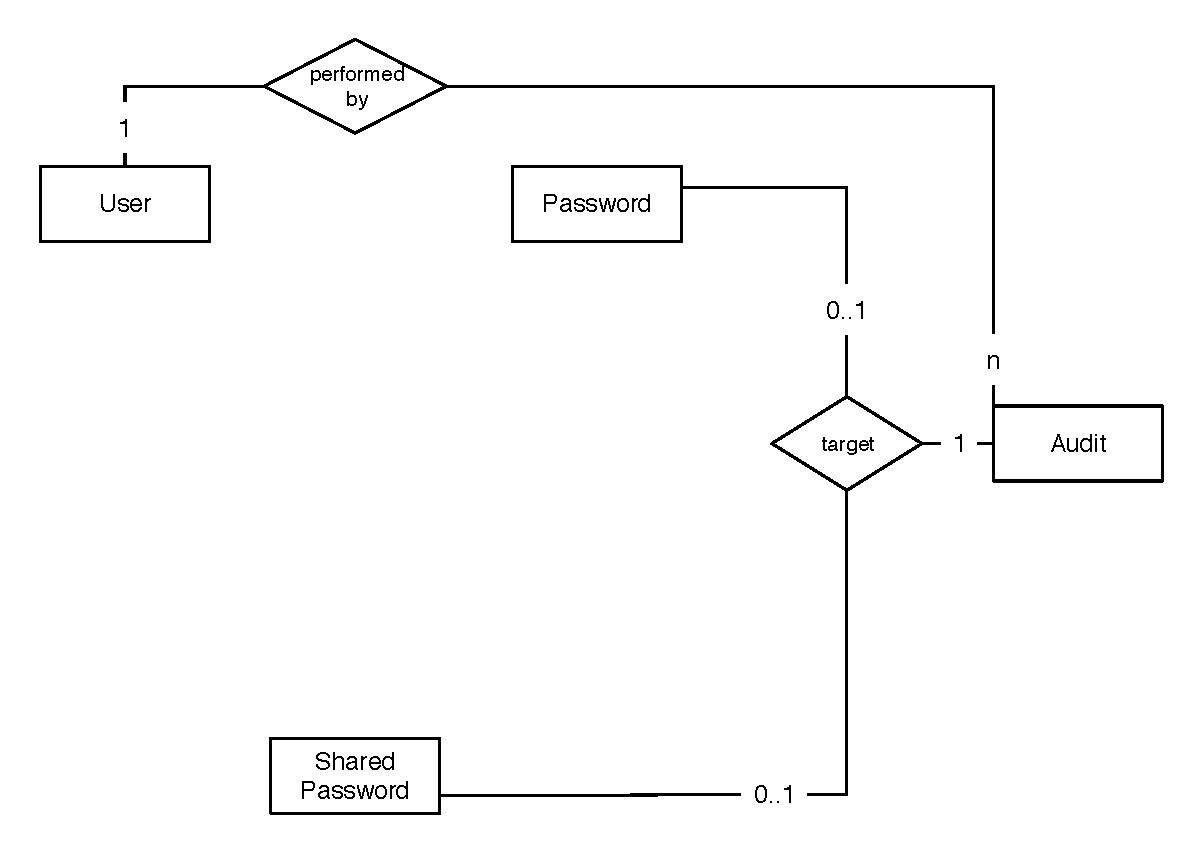
\includegraphics[width=\textwidth]{figures/design/uml/audit-user-password-shared-password-erd.eps}
				\caption{The Audit model's relationship with the User, Password, and Shared Password models.}
				\label{fig:relationship:audit-user}
			\end{figure}

		\subsection{Combining the Models}
			In the previous sections, the various models have been described and their relationships have been covered using Entity Relationship diagrams. Finally, all of these diagrams are combined into a single one, representing the entire system. This is found on figure \ref{fig:erd:full} on page \pageref{fig:erd:full}.

			\begin{figure}[p]
				\centering
				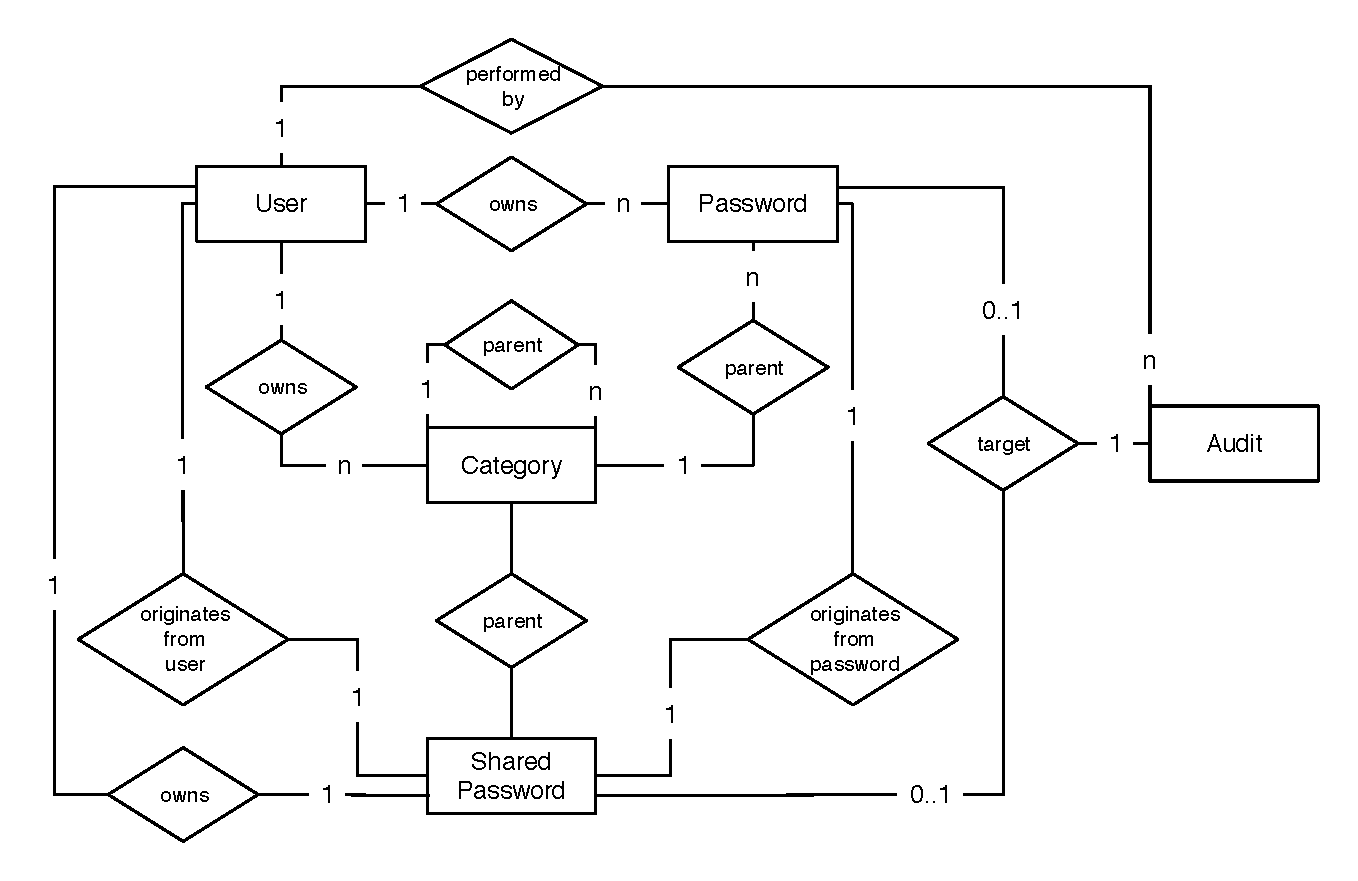
\includegraphics[width=\textwidth]{figures/design/uml/erd-full.eps}
				\caption{Entity Relationship Diagram for the System, using Chen's notation.}
				\label{fig:erd:full}
			\end{figure}

		\subsection{Comparison With Requirements}
			\label{requirement:fulfilled:organization}
			\label{requirement:fulfilled:new}
			\label{requirement:fulfilled:retrieve}
			\label{requirement:fulfilled:delete}


			Having modelled the core compon

			Section \ref{sec:model:category} on page \pageref{sec:model:category} introduced the concept of the Category model. This model allows for near infinite structuring of the password storage. As such, it is concluded that the solution fulfil functional requirement \#\ref{requirement:organization}:
			\vspace{-3ex}\begin{enumerate}
				\setlength\itemsep{0.1em}
				\setcounter{enumi}{4-1}
				\item Password organisation, multiple levels
			\end{enumerate}

			Additionally, section \ref{sec:model:password} on page \pageref{fig:model:password} described the model of each password entry. As such, it is concluded that the solution fulfil functional requirements \#\ref{requirement:new}, \#\ref{requirement:retrieve}, and \#\ref{requirement:delete}:
			\vspace{-3ex}\begin{enumerate}
				\setlength\itemsep{0.1em}
				\setcounter{enumi}{10-1}
				\item Support adding of new passwords
				\item Support retrieving stored passwords
				\item Support deleting stored passwords
			\end{enumerate}
	\section{Storing the Data}
		Up until now the phrase ``database'' has been used as a generic description of persistent storage. In this section, this will be elaborated a bit. Generally speaking, there primarily exist two categories of databases: Relational Database Management Systems \emph{(RDBMSs)} and Non-SQL \emph{(NoSQL)}

		RDBMS/SQL is the oldest of the bunch. This category covers the first database schemes ever used, dating back to the 70's. This type of database has a very strict structure, compared to the others, requiring a structure of tables, which in turn contains columns. RDBMS are by far, the most used type of database, if for no other reason, that they've simply existed for a lot longer. Typically RDBMSs uses the Structured Query Language \emph{(SQL)}. An example of a RDBMS table can be seen on table \ref{fig:example:rldb} on page \pageref{fig:example:rldb}, consisting of columns ID, Username, and E-Mail, each entry has one value for each column. RDBMS often adhere to the ACID qualities: Atomic, Consistent, Isolated, and Durable. These ensures that either a query succeeds or it fails. Additionally, most implementations support transactions. Transactions work by effectively grouping several queries. The smart thing about this, is that either the transaction fails, or it succeeds. I.e. either all of the sub-queries succeeds, or if \emph{one} of them fails, all of the changes are rolled back.

		\begin{table}[h!]
			\centering
			\begin{tabular}{|c|c|c|}
				\hline
				\textbf{ID} 		& 	\textbf{Username} 		& \textbf{E-Mail} 		\\
				\hline
				1 					& Daniel 					& some@mail.com 		\\
				\hline
				2 					& John 						& someother@mail.com 	\\
				\hline
				3 					& Kylo Ren 					& kren@firstorder.com 	\\
				\hline
			\end{tabular}
			\caption{RDBMS table example}
			\label{fig:example:rldb}
		\end{table}

		While generally NoSQL is being used to describe a set of implementations, much like RDBMS is. However, this is not exactly true. There exists no standard for NoSQL databases, and each implementation varies greatly, which unfortunately results in the various implementations API's being vastly different from each other.

		NoSQL databases uses JSON format to represent information in the database. Where as SQL entries are restricted to the columns in the table, NoSQL does not have this constraint. The example from before, is stored as follows, using the JSON syntax. An example of this is found on listing \ref{lst:example:nosql} on page \pageref{lst:example:nosql}. One of the advantages of NoSQL is that since it does not have a strict schema, additional values can easily be added, for instance, it would be perfectly fine if a fourth user was added to the example, containing a field called phone. Where RDBMS adhere to ACID, NoSQL adhere to BASE: Basic Availability, Soft-state, and Eventual consistency.

		\begin{lstlisting}[style=json2,gobble=8, caption={NoSQL table example},label={lst:example:nosql}]
        [
            {
                "ID": 1,
                Username: Daniel,
                E-Mail: some@mail.com
            },
            {
                ID: 2,
                Username: John,
                E-Mail: someother@mail.com
            },
            {
                ID: 3,
                Username: Kylo Ren,
                E-Mail: kren@firstorder.com
            }
        ]
		\end{lstlisting}

		First and foremost, it is important to realise that \emph{all} of the technologies are capable of storing what is required. Having said that, one of the most credited advantages of NoSQL is their ability to scale horizontally. It can be spread out over multiple hosts, if need be. However, this project \emph{should} never reach that size. It is not intended to reach that size. As such, that advantage can be disregarded.

		At this point in time, tables such as \cite{db_rankings} could be used to argue that one type of database generally is faster. However, this really wouldn't matter much, in the context of this project. This is \emph{meant} to be self-hosted. It is \emph{meant} to be used by individuals. As such, it is \emph{highly} unlikely, that this project would ever find itself in a situation, where millions of records are being queried constantly. It would simply not make much sense, to use these arguments.

		But what then. In section \ref{sec:modelling} on page \pageref{sec:modelling}, the contents of the various models were discussed. The way it was designed, hints heavily at a underlying relational scheme. The audit entries, for instance, is a \emph{perfect} example of where a relational database would excel. Furthermore, there is the issue of invites. The process of using an invite would most likely involve something like the following steps:
		\begin{enumerate}
			\item Check that the invite exists
			\item Check that the invite is not expired
			\item Use the invite to create new user
			\item Delete invite
		\end{enumerate}
		However, as should be \emph{obvious} to everyone, this will be painfully vulnerable to race-conditions. This \emph{exact} scenario, is completely mitigated by the use of RDBMSs transactions: These would make the four steps atomic, in the eyes of the database. While some NoSQL databases adhering to the ACID principles, and supporting transactions, are starting to appear\cite{no_sql_transactions}, it is by far all of them that supports this.

		As such, it is decided that a more ``traditional'' RDBMS will be used for this solution.

		\subsection{Being Database Agnostic}
			As written in the requirements, cf. section \ref{sec:requirements}, the solution should be database agnostic. In the previous paragraphs, it has been determined that the solution should use a RDBMS.

	\section{Ensuring Agnosticism}
		\todo{Explain platform agnositicms}
		\todo{explain need cross platform solution}
		\todo{explain need for database abstraction layer}
	\section{Licensing the Solution}
		Use MIT YO!
		\todo{Explain MIT license}

	\section{Final Comparison with the Requirements}
		\begin{table}[h!]
			\begin{tabular}{r l c}
												& \rot{\textbf{Fulfilled}} 	& \rot{Section} \\
				\textbf{Functional} 			&						&					\\
				\hline
				\freq{item:distrib_password} 	& \green{\cmark} 			& \green{ \ref{requirement:fulfilled:distrib_password} }			\\
				\hline
				\freq{item:multi_user} 			& \green{\cmark} 			& \green{ \ref{requirement:fulfilled:multi_user} }			\\
				\hline
				\freq{item:admin_user} 			& \green{\cmark} 			& \green{ \ref{requirement:fulfilled:admin_user} }			\\
				\hline
				\freq{item:organization} 		& \green{\cmark} 			& \green{ \ref{requirement:fulfilled:organization} }			\\
				\hline
				\freq{item:sharing} 			& \green{\cmark} 			& \green{ \ref{requirement:fulfilled:sharing} }			\\
				\hline
				\freq{item:add} 			 	& \green{\cmark} 			& \green{ \ref{requirement:fulfilled:add} }			\\
				\hline
				\freq{item:platform} 			& \red{\xmark} 			& \red{ }			\\
				\hline
				\freq{item:database} 			& \red{\xmark} 			& \red{ }			\\
				\hline
				\freq{item:passwords_local} 	& \green{\cmark} 			& \green{ \ref{requirement:fulfilled:passwords_local} }			\\
				\hline
				\freq{item:new} 				& \green{\cmark} 			& \green{ \ref{requirement:fulfilled:new} }			\\
				\hline
				\freq{item:retrieve} 			& \green{\cmark} 			& \green{ \ref{requirement:fulfilled:retrieve} }			\\
				\hline
				\freq{item:delete} 				& \green{\cmark} 			& \green{ \ref{requirement:fulfilled:delete} }			\\
				\hline
				\freq{item:audit} 				& \green{\cmark} 			& \green{ \ref{requirement:fulfilled:audit} }			\\
				\hline
				\freq{item:auth} 				& \green{\cmark} 			& \green{ \ref{requirement:fulfilled:auth} }			\\
				\hline
				\freq{item:change} 				& \green{\cmark} 			& \green{ \ref{requirement:fulfilled:change} }			\\
				\hline
				\freq{item:two-factor} 			& \green{\cmark} 			& \green{ \ref{requirement:fulfilled:two-factor} }			\\
				\hline
				\freq{item:restart} 			& \red{\xmark} 			& \red{ }			\\
				\hline
				\textbf{Non-Functional} 		&  			 			& 					\\
				\hline
				\nfreq{item:user_storage} 		& \red{\xmark} 			& \red{ }			\\
				\hline
				\nfreq{item:open-source} 		& \red{\xmark} 			& \red{ }			\\
				\hline
				\nfreq{item:entries} 			& \red{\xmark} 			& \red{ }			\\
				\hline
				\nfreq{item:encryption} 		& \green{\cmark} 			& \green{ \ref{requirement:fulfilled:encryption} }			\\
				\hline
				\nfreq{item:comms} 				& \green{\cmark} 			& \green{ \ref{requirement:fulfilled:comms} }	\\
				\hline
				\nfreq{item:tls1.2} 			& \red{\xmark} 			& \red{ }			\\
				\hline
				\nfreq{item:delay} 				& \red{\xmark} 			& \red{ }			\\
				\hline
			\end{tabular}
		\end{table}